\chapter{\babDua}
\label{bab:tinjauan}
\hyphenation{FastAPI SQLite SQLAlchemy Pydantic Starlette statsmodels mlxtend NumPy JavaScript Playwright Laravel Starbucks ihelon es-pre-so eks-trak-si ren-de-men pe-nye-duh-an pen-ska-la-an re-ko-men-da-si per-se-di-a-an pe-ra-mal-an a-so-si-a-si ba-ris-ta ta-kar-an stan-dar-di-sa-si re-frak-to-me-ter kon-ver-si da-ta-set back-end front-end frame-work end-point re-stock sup-port con-fi-dence le-ver-age con-vic-tion boot-strap base-line smooth-ing boost-ing sea-son-al for-ward chain-ing us-abil-ity ac-cep-tance bound-ary par-ti-tion-ing equiv-a-lence mi-cro-foam in-ven-to-ri pe-la-tih-an pem-ban-ding pe-ngem-bang-an}
% Hindari pemenggalan yang menyisakan dua huruf (misalnya "-an") di awal baris; dikembalikan di akhir bab.
\edef\babDuaRightHyphenMin{\the\righthyphenmin}
\righthyphenmin=3

% Sumber fakta bab ini: tools/PANDUAN_PENULISAN.md, app/SPEC.md, "Skripsi Arahan Pak Budi.pdf",
% referensi_terverifikasi.json (setiap klaim dicocokkan dengan abstract_evidence sumbernya) dan
% rumus_terverifikasi.json (hanya entri berstatus confirmed; kunci sitasi mengikuti field cite).
% Rumus yang dirumuskan penulis ditandai eksplisit di teks. Bab ini tidak memuat angka hasil evaluasi.
% Gambar pic/bagan_kendali_seduh.png dan pic/rolling_origin.png dibuat dengan tools/gambar_bab2.py.

Bab ini menyajikan teori dan penelitian terdahulu yang menjadi dasar perancangan aplikasi Takar pada Bab~\ref{bab:metode}. Subbab~\ref{sec:landasan-teori} membahas konsep yang dipakai pada bab-bab berikutnya, Subbab~\ref{sec:penelitian-terkait} membandingkan penelitian terapan yang paling dekat dan merumuskan kesenjangan yang diisi penelitian ini, dan Subbab~\ref{sec:kerangka-pemikiran} merangkum alur pemikiran dari masalah hingga hipotesis. Setiap konsep dikaitkan dengan bagian aplikasi Takar yang memakainya agar hubungan antara teori dan rancangan pada Bab~\ref{bab:metode} terlihat jelas. Persamaan bernomor hanya memuat rumus yang tercetak atau didefinisikan pada sumber yang disitasi; rumus yang dirumuskan penulis ditandai secara eksplisit.

%=============================================================================%
\section{Landasan Teori}
\label{sec:landasan-teori}

Landasan teori disusun mengikuti alur kerja Takar. Pengetahuan kopi dan resep menjadi basis pengetahuan, penskalaan dan persediaan menjadi logika inti, aplikasi web menjadi wadahnya, dan kecerdasan buatan menjadi lapisan rekomendasi di atasnya, sedangkan metode pengembangan dan pengujian melengkapi keempatnya. Subbab~\ref{subsec:kedai-kopi}--\ref{subsec:persediaan} membahas domain kopi serta logika takaran dan stok, dan Subbab~\ref{subsec:sistem-web} membahas teknologi aplikasi. Subbab~\ref{subsec:kecerdasan-buatan}--\ref{subsec:evaluasi-rekomendasi} membahas kecerdasan buatan beserta evaluasinya, sedangkan Subbab~\ref{subsec:scrum}--\ref{subsec:pengujian} membahas metode pengembangan dan pengujian.

%-----------------------------------------------------------------------------%
\subsection{Industri Kedai Kopi, Resep Standar, dan SOP}
\label{subsec:kedai-kopi}

Dalam penelitian ini, kedai kopi (\textit{coffee shop}) dipahami sebagai usaha jasa makanan dan minuman yang menyajikan minuman kopi yang diracik barista di area bar. Laporan \textit{Coffee Annual} untuk Indonesia mencatat bahwa kopi susu tetap menjadi minuman pengantar yang populer di kedai kopi \citep*{rahmanulloh2026coffee}, dan kualitas produk serta layanan berpengaruh positif terhadap kepuasan dan niat beli ulang pelanggan sebuah kedai kopi di Bali \citep*{natalia2023role}. Karena itu, minuman yang sama harus disajikan dengan takaran, parameter, dan hasil yang sama dari cangkir ke cangkir dan dari \textit{shift} ke \textit{shift}. Konsistensi ini tidak tercapai dengan sendirinya: kopi seduhan barista manusia menunjukkan variasi senyawa volatil yang lebih besar daripada seduhan robot barista \citep{park2023robot}, dan pada seduhan filter, tekanan serta turbulensi saat barista menuang air menjadi variabel kunci reprodusibilitas \citep{santanatoglia2023impact}. Studi yang sama juga menemukan reprodusibilitas kekuatan seduhan (TDS) dan waktu seduh yang sangat baik pada seduhan V60 dan Pure Brew dari enam barista ahli, sehingga konsistensi yang tinggi dapat dicapai oleh barista yang terampil. Restoran berantai dapat memusatkan produksi di dapur sentral; menurut model analitis \citet*{zhang2025improving}, menguntungkan atau tidaknya investasi itu bergantung pada sensitivitas pelanggan terhadap inkonsistensi mutu. Kedai kopi meracik minuman saat dipesan, sehingga standardisasi harus dilakukan langsung di bar.

Resep standar adalah panduan untuk menyiapkan suatu makanan atau minuman secara konstan pada mutu yang diharapkan \citep*{naumov2023employment}. Unsurnya adalah nama resep, hasil (\textit{yield}), ukuran porsi, berat atau jumlah, takaran atau satuan, bahan, instruksi, dan catatan, sehingga mutu, kuantitas, dan biaya porsi dapat diprediksi dan dikendalikan; penulis yang sama juga berargumen secara konseptual bahwa resep standar mempercepat pelatihan karyawan. Buku ajar kuliner \citet*{gisslen2025professional} membahas resep standar bersama pengukuran bahan, pengendalian porsi, satuan ukur, serta konversi resep dan masalahnya. Agar dapat diolah komputer, resep perlu disimpan secara terstruktur, karena frasa bahan dalam teks bebas sangat bervariasi sehingga nama, satuan, dan jumlahnya sulit diekstrak secara tepat \citep*{shi2022attention}; satuan ukur juga perlu dimodelkan secara eksplisit agar data kuantitatif dapat diintegrasikan, diverifikasi, dan direproduksi \citep*{rijgersberg2013ontology}. Komposisi yang terstruktur dapat diperlakukan sebagai daftar bahan (\textit{bill of materials}, BOM). \citet{kamal2021bill} mengusulkan analisis BOM menu karena analisis manual atas bahan penyusun menu yang kompleks tidak efisien, dan \textit{dataset} \citet*{zolfagharnasab2024coffee} memberi contoh BOM 40 produk kedai kopi, misalnya Latte dengan 22~g biji espreso, 60~ml air, dan 180~ml susu. Pada Takar, BOM dipakai untuk memotong stok ketika produksi dicatat dan untuk menurunkan ramalan penjualan menu menjadi kebutuhan bahan (Subbab~\ref{subsec:persediaan}).

Prosedur operasional standar (\textit{standard operating procedure}, SOP) dirancang untuk memastikan konsistensi, efisiensi, mutu, dan kepatuhan kegiatan operasional; pada sebuah kafe di Jember, unsur SOP yang efisien, efektif, dan konsisten berpengaruh signifikan terhadap kualitas pelayanan menurut pelanggannya \citep*{chapitoline2024pengaruh}. SOP Takar terdiri atas SOP resep, yaitu langkah penyajian setiap resep arahan, dan SOP umum seperti kalibrasi espreso, \textit{steaming} susu, serta pembukaan dan penutupan bar. SOP yang ditampilkan saat bekerja berfungsi sebagai alat bantu kerja (\textit{job performance aid}, JPA), yaitu alternatif atau pelengkap pelatihan yang hemat biaya yang menyimpan rincian penting untuk dipakai sesaat sebelum atau selama tugas, efektif selama mengurangi hal yang harus diingat dan merinci tindakan beserta waktunya, dan berbentuk panduan prosedural, lembar kerja, daftar periksa, tabel keputusan, atau diagram alir \citep*{campbell1996job}. Panduan seduh bertahap Takar termasuk panduan prosedural, daftar periksa SOP termasuk daftar periksa, dan tabel aturan sistem pakar menyerupai tabel keputusan. Alat bantu semacam ini relevan karena pekerjaan barista merupakan jalinan kerumitan operasional dengan keterampilan yang berkembang sebagai kebiasaan \citep*{lee2022barista}, dan sistem realitas virtual yang memberi umpan balik korektif dilaporkan meningkatkan kinerja belajar mahasiswa yang berlatih menyeduh \textit{pour over} \citep*{yu2021developing}. Penulis berpendapat bahwa resep standar dan pencatatan stok dapat membantu mencegah limbah pangan, karena pada lima studi kasus jasa makanan di Malaysia, hampir sepertiga makanan terbuang dan penyebabnya mencakup prosedur serta kebijakan operasional gerai \citep{papargyropoulou2019patterns}.

%-----------------------------------------------------------------------------%
\subsection{Ilmu Penyeduhan Kopi}
\label{subsec:penyeduhan}

Menyeduh kopi berarti mengekstrak senyawa terlarut dari kopi sangrai giling ke dalam air. Metode seduh berbeda dalam tekanan ekstraksi, rasio kopi dan air, kualitas air, waktu kontak, distribusi ukuran partikel, dan suhu; seluruh parameter tersebut mengubah ekstraksi senyawa yang membentuk cita rasa \citep*{cordoba2020coffee}. Partikel kecil terekstraksi lebih cepat daripada partikel besar \citep{uman2016effect}, sehingga ukuran gilingan menjadi salah satu tuas untuk mengubah laju ekstraksi, walaupun di bawah ukuran gilingan kritis ekstraksi justru dapat turun karena aliran di dalam ampas tidak seimbang \citep*{lee2023uneven}. Subbab ini membahas ukuran ekstraksi dan bagan kendali seduh, lalu parameter espreso, \textit{pour over} V60, dan susu yang dipakai resep arahan.

\subsubsection{Rasio Seduh, TDS, dan Rendemen Ekstraksi}
\label{subsubsec:tds-ey}

Rasio seduh (\textit{brew ratio}) didefinisikan sebagai massa air seduh dibagi massa kopi giling \citep*{liang2021equilibrium}:
\begin{equation}
R_{\mathrm{brew}} = \frac{M_w}{M_g},
\label{eq:rasio-seduh}
\end{equation}
dengan $R_{\mathrm{brew}}$ rasio seduh tak berdimensi, $M_w$ massa air seduh (g), dan $M_g$ massa kopi giling atau dosis (g). Orientasi yang sama dipakai \citet{guinard2023new}. Resep V60 pada arahan, yaitu 15~g kopi untuk 225~ml air (``1:15''), memberi $R_{\mathrm{brew}} = 15$ bila 1~ml air dianggap bermassa 1~g. Standar industri kadang memakai orientasi sebaliknya, misalnya 55~g kopi per 1~kg air pada SCA 310-2021 \citep*{sca2022home}, sehingga skripsi ini selalu menyebut orientasi rasio yang dipakai. Pada seduhan imersi penuh, TDS kira-kira berbanding terbalik dengan rasio air terhadap kopi, sedangkan rendemen ekstraksi hampir tidak bergantung pada rasio, sehingga rasio seduh menjadi parameter terpenting \citep*{liang2021equilibrium}; bagi V60 yang merupakan seduhan perkolasi, hubungan ini hanya berlaku sebagai pendekatan.

Kekuatan seduhan diukur sebagai padatan terlarut total (\textit{total dissolved solids}, TDS), yaitu fraksi massa padatan kopi yang terlarut di dalam cairan seduhan \citep*{liang2021equilibrium, batali2020brew}:
\begin{equation}
\mathrm{TDS} = \frac{M_d}{M_L},
\label{eq:tds}
\end{equation}
dengan $M_d$ massa padatan kopi terlarut (g) dan $M_L$ massa cairan yang mengandungnya (g). TDS biasanya dilaporkan dalam persen dan ditaksir dengan refraktometer kopi \citep*{sca2022home}. Rendemen ekstraksi (\textit{extraction yield}, EY), yang juga disebut \textit{percent extraction} (PE), menyatakan proporsi massa kopi giling yang berpindah ke dalam minuman \citep*{batali2020brew}:
\begin{equation}
\mathrm{EY} = \mathrm{TDS} \times \frac{M_{\mathrm{bev}}}{M_{\mathrm{dose}}},
\label{eq:ey}
\end{equation}
dengan $M_{\mathrm{bev}}$ massa minuman (g) dan $M_{\mathrm{dose}}$ massa kopi giling (g). Bentuk yang sama dipakai untuk espreso, yang resepnya lazim dinyatakan sebagai dosis masuk dan hasil keluar, misalnya 18~g kopi menghasilkan 36~g minuman \citep{moroney2019analysing}.

Pada seduhan perkolasi, sebagian air tertahan di ampas basah sehingga massa minuman lebih kecil daripada massa air. \citet{guinard2023new} menuliskan neraca massa yang mengaitkan PE, TDS, dan rasio seduh dengan koreksi untuk air tertahan tersebut:
\begin{equation}
\mathrm{PE} = \frac{\mathrm{TDS}}{1 - \mathrm{TDS}}\left(R_{\mathrm{brew}} - R_{\mathrm{abs}}\right), \qquad R_{\mathrm{abs}} \approx 2{,}1,
\label{eq:neraca-massa}
\end{equation}
dengan PE dan TDS dalam bentuk fraksi dan $R_{\mathrm{abs}}$ rasio penyerapan (\textit{liquid retention ratio}), yaitu massa air yang tertahan pada ampas per massa kopi. Bila $R_{\mathrm{abs}} = 0$, persamaan ini menjadi neraca massa seduhan imersi penuh \citep*{liang2021equilibrium}. Persamaan~\eqref{eq:neraca-massa} memungkinkan PE ditaksir dari rasio dan TDS tanpa menimbang minuman. Untuk V60 arahan ($R_{\mathrm{brew}} = 15$) dan $R_{\mathrm{abs}} = 2{,}1$, perhitungan penulis menunjukkan bahwa PE 18--22\% bersesuaian dengan TDS sekitar 1,38--1,68\%.

\subsubsection{Bagan Kendali Seduh dan Standar \texorpdfstring{\textit{Golden Cup}}{Golden Cup}}
\label{subsubsec:bagan-kendali}

Bagan kendali seduh (\textit{Coffee Brewing Control Chart}) dari tahun 1950-an memetakan TDS terhadap PE dan memberi label wilayah seperti ``\textit{underdeveloped}'', ``\textit{bitter}'', dan ``\textit{ideal}'' \citep*{frost2020effects}. Standar \textit{Golden Cup} dari Specialty Coffee Association of America (SCAA) menetapkan kekuatan seduhan 11,5--13,5~g/l, setara 1,15--1,35\% pada bagan, yang dihasilkan dari rendemen ekstraksi 18--22\%, serta merekomendasikan rasio kopi terhadap air 55~g/l $\pm$ 10\% dan suhu air 93,0 $\pm$ 3~$^\circ$C \citep*{scaa2015golden}. Standar SCA 310-2021 memakai target kekuatan yang lebih lebar, 1,15--1,55\%, dengan suhu campuran kopi dan air 90--96~$^\circ$C \citep*{sca2022home}. Rendemen 18--22\% juga diterima luas untuk espreso; seduhan di bawahnya (kurang terekstraksi) cenderung kurang beraroma dan dapat terasa terlalu asam, sedangkan seduhan di atasnya (terlalu terekstraksi) dapat terasa terlalu pahit \citep{moroney2019analysing}.

Gambar~\ref{fig:bagan-kendali} digambar penulis dari rentang \textit{Golden Cup} \citep*{scaa2015golden}, batas atas SCA 310-2021 \citep*{sca2022home}, dan Persamaan~\eqref{eq:neraca-massa} \citep{guinard2023new}. Batas \textit{Golden Cup} membagi bidang bagan menjadi sembilan zona: menurut TDS, seduhan dapat encer, ideal, atau pekat, dan menurut EY, seduhan dapat kurang terekstraksi, ideal, atau terlalu terekstraksi. Garis miring adalah rasio seduh tetap. Garis $R = 15$ untuk V60 arahan melintas di atas kotak \textit{Golden Cup}, dan konsentrasinya, $15/0{,}225 \approx 66{,}7$~g/l, berada di atas rentang 49,5--60,5~g/l yang dihitung penulis dari rekomendasi 55~g/l $\pm$ 10\%. Artinya, bila EY-nya berada pada rentang ideal 18--22\%, V60 yang diseduh tepat menurut arahan akan terbaca pekat pada bagan klasik, tetapi tetap di bawah batas atas SCA 310-2021 selama EY-nya tidak melebihi sekitar 20\% (perhitungan penulis). Penelitian ini tetap memakai resep arahan sebagai standar kedai dan memperlakukan perbedaan itu sebagai keterangan pada sistem pakar, bukan sebagai kesalahan resep.

\begin{figure}[htbp]
\centering
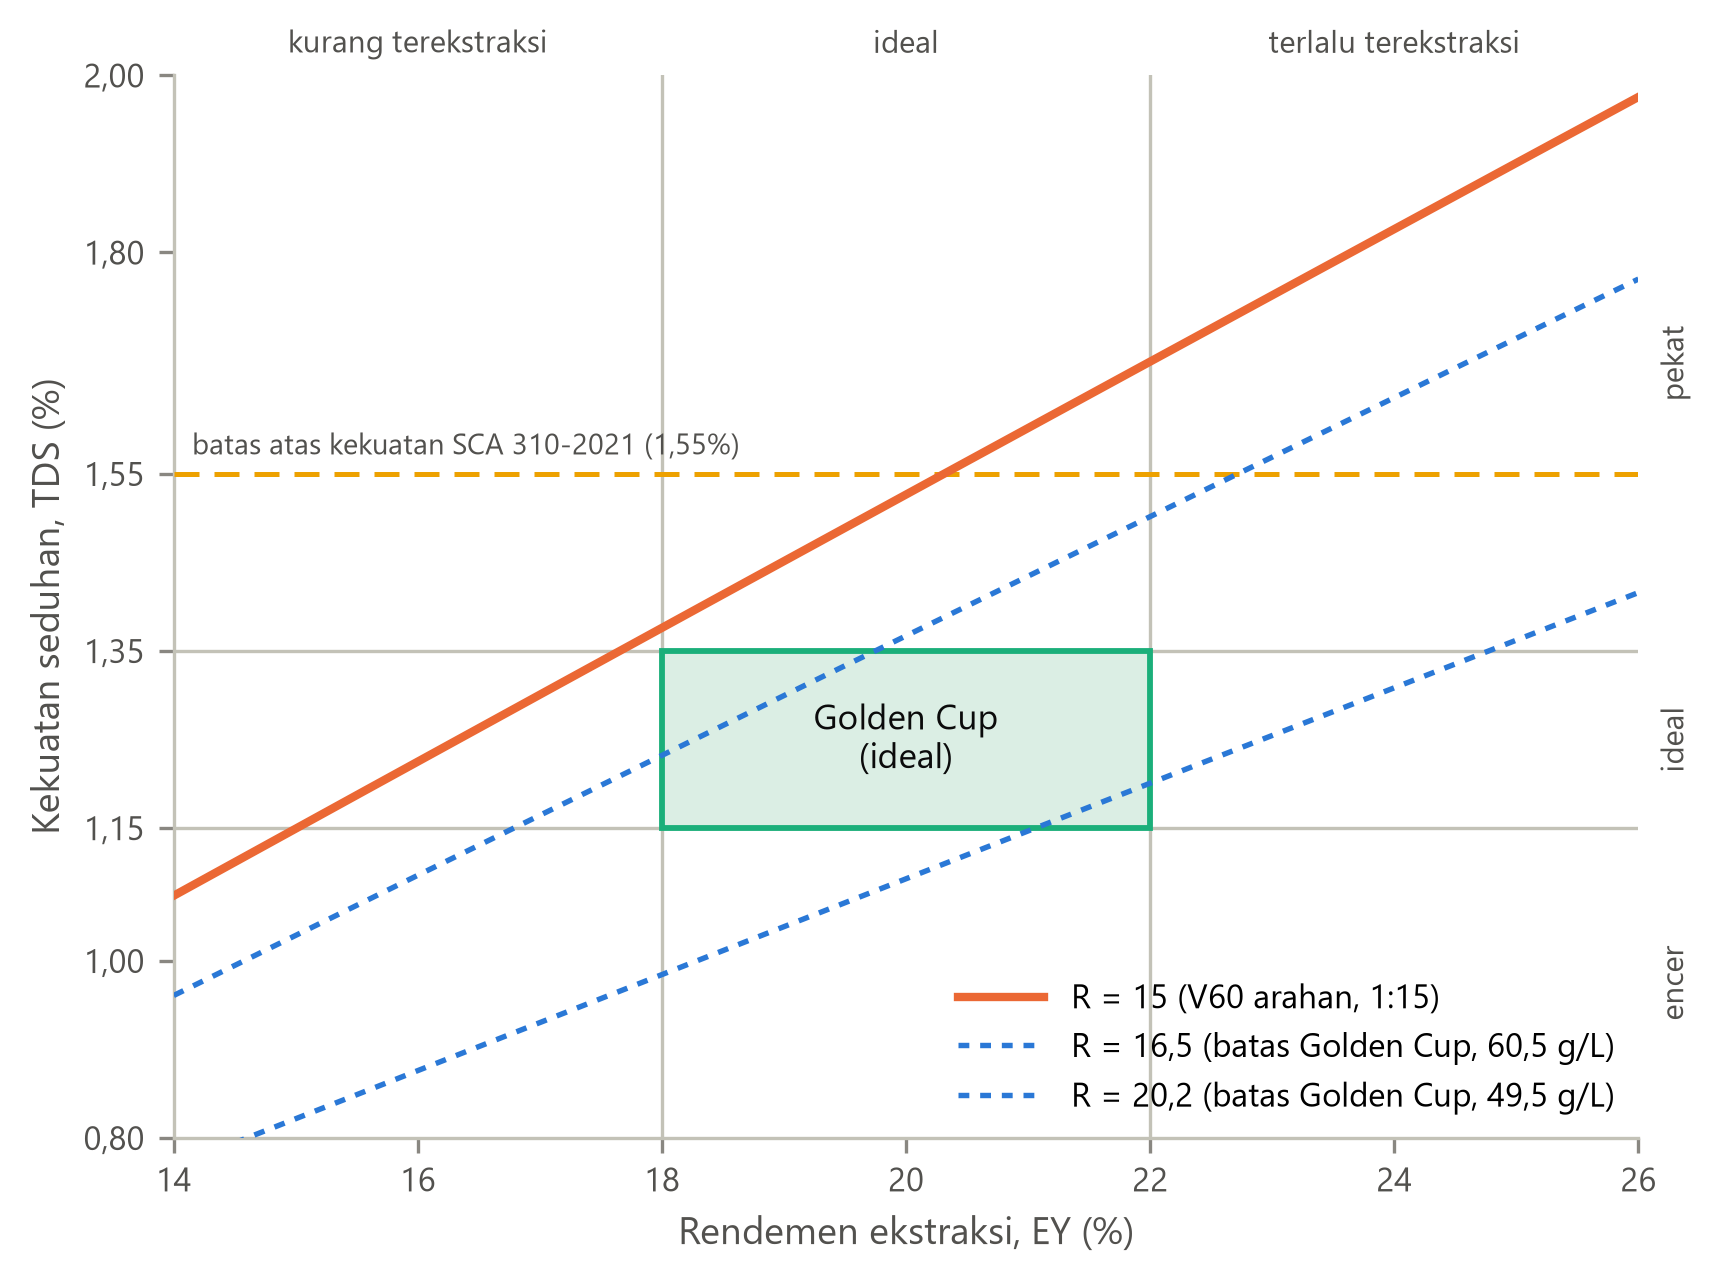
\includegraphics[width=0.78\textwidth]{pic/bagan_kendali_seduh.png}
\caption{Bagan Kendali Seduh dengan Kotak \textit{Golden Cup} dan Garis Rasio Seduh}
\label{fig:bagan-kendali}
\end{figure}

Kotak ideal bukan batas mutlak. Pada kopi tetes dengan sembilan kombinasi TDS dan PE, 21 dari 30 atribut sensori berbeda nyata antarseduhan dan rasa manis berbanding terbalik dengan TDS \citep*{frost2020effects}. Preferensi 118 konsumen kopi hitam tersebar pada rentang kekuatan dan rendemen yang lebar dan membentuk dua segmen yang preferensinya paling dipengaruhi TDS \citep*{cotter2020consumer}, dan rasa asam berkorelasi kuat dengan keasaman tertitrasi yang berkorelasi linier dengan TDS \citep*{batali2021titratable}. Sintesis studi-studi tersebut menghasilkan bagan kendali seduh versi baru, yaitu bagan sensori, bagan konsumen dengan dua klaster preferensi, gabungan keduanya, dan bagan ringkas \citep{guinard2023new}. Suhu air ternyata kurang menentukan: pada kopi tetes dengan target TDS dan PE yang sama pada 87, 90, dan 93~$^\circ$C, suhu seduh tidak berdampak berarti terhadap profil sensori \citep*{batali2020brew}. Karena itu, koreksi seduhan pada sistem pakar Takar diarahkan lebih dahulu ke TDS dan EY melalui rasio, gilingan, dan waktu kontak, dengan suhu air sebagai tuas terakhir.

\subsubsection{Espreso}
\label{subsubsec:espreso}

Espreso dibuat dengan mendorong air panas bertekanan melalui kopi giling halus yang dipadatkan. \citet{cameron2020systematically} menyebutnya sebagai format kopi yang paling rentan terhadap variasi: rendemennya memuncak pada pengaturan gilingan tertentu dan turun pada gilingan yang sangat kasar maupun halus; penurunan pada gilingan halus mereka tafsirkan sebagai petunjuk kuat adanya aliran tidak homogen yang menurunkan reprodusibilitas dan membuang bahan baku. \citet*{schmieder2023influence} mendefinisikan rasio seduh espreso sebagai perbandingan massa kopi giling di dalam \textit{puck} terhadap massa espreso yang terekstraksi ke cangkir:
\begin{equation}
\mathrm{BR} = \frac{m_{\mathrm{kopi}}}{m_{\mathrm{espreso}}},
\label{eq:rasio-espreso}
\end{equation}
dengan $m_{\mathrm{kopi}}$ dosis kopi giling (g) dan $m_{\mathrm{espreso}}$ massa espreso di cangkir (g). Dengan definisi ini, \textit{ristretto} memiliki BR 1/1, espreso BR 1/2, dan \textit{lungo} BR 1/3. Orientasinya berlawanan dengan Persamaan~\eqref{eq:rasio-seduh}, sehingga kedua besaran tidak boleh dicampur; Takar menyimpan kebalikannya, yaitu rasio hasil $1/\mathrm{BR}$ yang bernilai 2 untuk espreso 1:2, sebagai konvensi penulis. Kekuatan espreso 8--12\% disebut tipikal, dan waktu ekstraksinya diatur dengan menghaluskan atau mengasarkan gilingan \citep{moroney2019analysing}. Pengaruh gilingan, laju alir, dan suhu terhadap massa komponen di dalam cangkir tergolong kecil dibandingkan pengaruh perbedaan massa total minuman yang diekstrak \citep*{schmieder2023influence}, dan bagan kendali seduh kinetik untuk espreso juga menunjukkan bahwa rasio seduh lebih berpengaruh terhadap komposisi kopi daripada suhu atau laju alir \citep*{pannusch2024modelbased}. Penulis menyimpulkan bahwa satu \textit{shot} espreso sebaiknya diperlakukan sebagai satuan resep yang tetap, sehingga ukuran minuman diubah dengan menambah atau mempertahankan jumlah \textit{shot} utuh (Subbab~\ref{subsec:penskalaan}). Arahan tidak menetapkan dosis, massa hasil, dan waktu ekstraksi espreso, sehingga nilainya ditetapkan sebagai asumsi pada Bab~\ref{bab:metode}; arahan hanya mengatur urutan tuang, yaitu air panas lebih dahulu pada Long Black agar \textit{crema} bertahan dan sebaliknya pada Americano.

\subsubsection{\texorpdfstring{\textit{Pour Over}}{Pour Over} V60 dan Susu}
\label{subsubsec:v60}

\textit{Pour over} adalah seduhan perkolasi manual: air dituang bertahap di atas kopi giling di dalam corong berkertas saring. Arahan menetapkan resep V60 untuk biji \textit{single origin} Gayo, Toraja, Flores, dan Ethiopia dengan 15~g kopi untuk 225~ml air, gilingan \textit{medium-fine}, dan suhu air 90--92~$^\circ$C, dengan tahapan \textit{blooming} 45~ml air yang didiamkan 30--45~detik untuk melepaskan karbon dioksida, penuangan melingkar hingga 130~ml pada menit ke-1:00, penuangan hingga 225~ml pada menit ke-1:30, dan penetesan yang selesai pada menit ke-2:30 sampai 3:00. Karena target tuangnya kumulatif, seluruh target harus ikut diskalakan ketika dosis berubah. Tabel~\ref{tab:parameter-seduh} membandingkan parameter arahan dengan literatur. Rentang praktik barista dan penyeduh rumahan di Cianjur yang memakai corong V60 menempatkan rasio 1:14--1:16 dengan waktu 2:30--3:00 pada gilingan \textit{medium} dan menyebut \textit{blooming} sekitar 30--45~detik \citep*{bramantoro2025optimization}, walaupun rentang dari sejumlah kecil seduhan itu merupakan bukti praktik, bukan standar. Untuk gilingan \textit{fine-medium}, yang paling dekat dengan gilingan \textit{medium-fine} pada arahan, sumber yang sama mencatat rasio 1:12--1:14, waktu 2--3~menit, dan suhu 86--88~$^\circ$C, sedangkan suhu 90--92~$^\circ$C hanya muncul pada gilingan \textit{medium-coarse}; kombinasi parameter arahan tidak sepadan dengan satu baris praktik tersebut. Gas yang dilepaskan saat \textit{blooming} berkaitan dengan CO\textsubscript{2} yang terbentuk saat sangrai dan dilepaskan lebih mendadak saat penggilingan dan ekstraksi \citep{smrke2017timeresolved}; kaitannya dengan langkah \textit{blooming} adalah inferensi penulis.

\begin{table}[!htb]
\centering
\caption{Parameter Penyajian pada Arahan dan Nilai Acuan dari Literatur}
\label{tab:parameter-seduh}
{\small
\setstretch{1.0}
\begin{tabular}{@{}>{\raggedright\arraybackslash}p{2.5cm}>{\raggedright\arraybackslash}p{3.5cm}>{\raggedright\arraybackslash}p{5.7cm}>{\raggedright\arraybackslash}p{1.3cm}@{}}
\toprule
\textbf{Parameter} & \textbf{Arahan Penelitian} & \textbf{Nilai Acuan} & \textbf{Sumber} \\
\midrule
\multicolumn{4}{@{}l}{\textit{V60 / pour over}} \\
Rasio seduh & 1:15 (15~g : 225~ml) & 55~g/l $\pm$ 10\%, setara 1:16,5--1:20,2\textsuperscript{a} & (1) \\
Suhu air & 90--92~$^\circ$C & 93,0 $\pm$ 3~$^\circ$C (air, SCAA); 90--96~$^\circ$C (campuran kopi dan air, SCA 310-2021) & (1), (2) \\
\textit{Blooming} & 45~ml, 30--45~detik & 30--45~detik & (3) \\
Waktu seduh & Selesai 2:30--3:00 & 2:30--3:00 (gilingan \textit{medium})\textsuperscript{b} & (3) \\
TDS; EY & Tidak ditetapkan & 1,15--1,35\% atau 1,15--1,55\%; 18--22\% & (1), (2) \\
\addlinespace
\multicolumn{4}{@{}l}{\textit{Espreso}} \\
Rasio seduh & Tidak ditetapkan & BR 1/2 (\textit{ristretto} 1/1, \textit{lungo} 1/3) & (4) \\
TDS; EY & Tidak ditetapkan & 8--12\% (tipikal); 18--22\% & (5) \\
\addlinespace
\multicolumn{4}{@{}l}{\textit{Susu}} \\
Suhu \textit{steaming} & 60--65~$^\circ$C & Optimum busa 50--60~$^\circ$C; nutrisi tidak terpengaruh pada 60--65~$^\circ$C & (6), (7) \\
Busa & Latte sekitar 1~cm; cappuccino 1,5--2~cm & Susu pasteurisasi membentuk busa lebih stabil daripada UHT & (6), (7) \\
\bottomrule
\end{tabular}}

\vspace{3pt}
{\footnotesize\raggedright Sumber: (1) \citet*{scaa2015golden}; (2) \citet*{sca2022home}; (3) \citet*{bramantoro2025optimization}; (4) \citet*{schmieder2023influence}; (5) \citet{moroney2019analysing}; (6) \citet{klimanova2022effect}; (7) \citet{santini2023effects}. \textsuperscript{a}\,Dihitung penulis dengan anggapan 1~ml air bermassa 1~g. \textsuperscript{b}\,Untuk gilingan \textit{fine-medium}, sumber (3) mencatat 1:12--1:14, 2--3~menit, dan 86--88~$^\circ$C; suhu 90--92~$^\circ$C hanya muncul pada gilingan \textit{medium-coarse}.\par}
\end{table}

Menurut arahan, Caffè Latte memakai susu segar yang di-\textit{steam} hingga 60--65~$^\circ$C sampai bertekstur lembut dengan \textit{microfoam} sekitar 1~cm, sedangkan Cappuccino memakai busa yang lebih tebal, sekitar 1,5--2~cm, di cangkir 150--180~ml. Busa susu dapat dilemahkan oleh lemak, fosfolipid, asam lemak bebas, dan gliserida parsial \citep*{huppertz2010foaming}. Pada \textit{steaming} dengan mesin espreso, busa dari susu utuh pasteurisasi cenderung lebih stabil dan suhu akhir optimumnya 50--60~$^\circ$C \citep{klimanova2022effect}, sedangkan mutu nutrisi susu tampak tidak terpengaruh pada 60--65~$^\circ$C tetapi menurun pada suhu yang lebih tinggi \citep{santini2023effects}. Rentang arahan dengan demikian sedikit melampaui suhu optimum busa, tetapi masih pada rentang yang tidak menurunkan mutu nutrisi, sehingga Takar tetap memakainya sebagai SOP kedai. Susu yang di-\textit{steam} bertambah volumenya karena busa, sehingga kalkulator memerlukan faktor ekspansi susu yang ditetapkan sebagai asumsi. Minuman dingin dan nonkopi menambahkan dua jenis pengetahuan: pengetahuan volume, misalnya Ice Brown Sugar Shaken Espresso yang berisi dua \textit{shot} espreso, 20~ml \textit{brown sugar syrup}, es batu secukupnya, dan susu hingga penuh (\textit{top up}); dan pengetahuan urutan, misalnya matcha pada Iced Matchagato yang dilarutkan lebih dahulu dengan air hangat agar tidak menggumpal dan Signature Pandan Latte yang disusun berlapis dengan espreso di atas. Pengetahuan pertama ditangani kalkulator penskalaan, sedangkan pengetahuan kedua disimpan sebagai langkah SOP.

%-----------------------------------------------------------------------------%
\subsection{Penskalaan Resep dan Faktor Konversi}
\label{subsec:penskalaan}

Penskalaan resep adalah penyesuaian takaran resep standar terhadap jumlah atau ukuran sajian yang berbeda dari resep asal, sedangkan hasil (\textit{yield}) menyatakan jumlah total yang dihasilkan resep. Cara yang paling umum adalah metode faktor konversi \citep*{bccook2015basic}:
\begin{equation}
f = \frac{Y_{\mathrm{butuh}}}{Y_{\mathrm{resep}}}, \qquad Y = n_{\mathrm{porsi}} \times s_{\mathrm{porsi}},
\label{eq:faktor-konversi}
\end{equation}
dengan $f$ faktor konversi, $Y_{\mathrm{butuh}}$ hasil yang dibutuhkan, $Y_{\mathrm{resep}}$ hasil resep asal, $n_{\mathrm{porsi}}$ jumlah porsi, dan $s_{\mathrm{porsi}}$ ukuran porsi. Setiap bahan kemudian dikalikan dengan faktor yang sama \citep*{bccook2015basic}:
\begin{equation}
q_i^{\mathrm{baru}} = f \times q_i^{\mathrm{asal}},
\label{eq:skala-linier}
\end{equation}
dengan $q_i^{\mathrm{asal}}$ dan $q_i^{\mathrm{baru}}$ takaran bahan ke-$i$ sebelum dan sesudah konversi; bentuk simbolik ini dituliskan penulis dari langkah prosedur dan tabel contoh pada sumber. Penelitian ini menyebut kedua persamaan tersebut sebagai penskalaan linier. Pada kalkulator Takar, $f$ adalah perbandingan volume cangkir tujuan terhadap cangkir dasar, atau perbandingan dosis baru terhadap dosis dasar untuk resep berbasis dosis seperti V60, sedangkan jumlah cangkir mengalikan takaran per cangkir.

Penskalaan linier sederhana, tetapi tidak selalu tepat. Sumber yang sama mengingatkan bahwa bumbu harus dinaikkan dengan hati-hati, waktu pengolahan dapat berubah bila peralatannya berbeda, dan penyesuaian halus hanya dapat dipelajari dari pengalaman, sehingga resep hasil konversi perlu diuji; cairan berkadar gula tinggi seperti sirup juga dianjurkan ditakar berdasarkan berat \citep*{bccook2015basic}. Bar kopi memiliki batasan khasnya sendiri, yang dirangkum penulis pada Tabel~\ref{tab:masalah-penskalaan}. Espreso diekstrak per \textit{shot} utuh, dan massa minuman espreso lebih menentukan komposisi di cangkir daripada gilingan, laju alir, dan suhu \citep*{schmieder2023influence}, sehingga faktor 1,25 tidak dapat dijalankan sebagai 1,25 \textit{shot}; pola ukuran menu sebuah jaringan kedai kopi besar juga bertingkat, bukan proporsional (Tabel~\ref{tab:pola-shot} pada Bab~\ref{bab:pendahuluan}). Susu yang diisi hingga penuh harus dikurangi ketika \textit{shot} ditambah agar minuman tidak meluap. Air dan target tuang V60 harus mengikuti dosis agar rasio 1:15 tetap, karena rasio seduh menentukan kekuatan seduhan \citep*{liang2021equilibrium}; dosis 20~g menuntut target tuang 60; 173,3; dan 300~ml. Hasil perkalian seperti 173,33~ml juga tidak dapat ditakar dengan alat di bar, dan pembulatan yang tidak konsisten membuat total beberapa cangkir berbeda dari jumlah takaran per cangkirnya.

\begin{table}[!htb]
\centering
\caption{Masalah Penskalaan Linier pada Resep Minuman Kopi}
\label{tab:masalah-penskalaan}
{\small
\setstretch{1.0}
\begin{tabular}{@{}>{\raggedright\arraybackslash}p{2.3cm}>{\raggedright\arraybackslash}p{3.4cm}>{\raggedright\arraybackslash}p{3.7cm}>{\raggedright\arraybackslash}p{3.6cm}@{}}
\toprule
\textbf{Masalah} & \textbf{Contoh dari Resep Arahan} & \textbf{Akibat Penskalaan Linier} & \textbf{Arah Penanganan} \\
\midrule
Bahan diskret & Caffè Latte: 1 \textit{shot}, cangkir 200--250~ml & Cangkir 200 ke 250~ml memberi $f = 1{,}25$, yaitu 1,25 \textit{shot} & \textit{Shot} dibulatkan ke \textit{shot} utuh atau mengikuti tabel ukuran \\
\addlinespace
Kapasitas cangkir & Ice Brown Sugar Shaken Espresso: susu \textit{top up} & Tambahan \textit{shot} tanpa mengurangi susu membuat minuman meluap & Susu dihitung sebagai sisa volume cangkir \\
\addlinespace
Rasio seduh & V60: 15~g : 225~ml; target tuang 45, 130, 225~ml & Rasio bergeser bila dosis dan air dibulatkan terpisah & Air dan target tuang dihitung dari dosis akhir dikali rasio \\
\addlinespace
Presisi takar & Sirup 20~ml, susu 150~ml & Takaran pecahan; total tidak sama dengan per cangkir dikali jumlah cangkir & Pembulatan ke presisi alat per cangkir, lalu dikalikan jumlah cangkir \\
\addlinespace
Pengubah pesanan & Kemanisan, tambahan \textit{shot}, penggantian susu atau biji & Pengubah ikut dikalikan faktor atau tidak menyesuaikan komponen lain & Pengubah diterapkan pada komponen sasarannya saja \\
\addlinespace
Es pada minuman dingin & Es batu ``secukupnya'' & Es tidak bertakaran dan volumenya tidak diperhitungkan & Massa es dan volumenya ditetapkan sebagai asumsi \\
\bottomrule
\end{tabular}}
\end{table}

Penanganan setiap masalah bergantung pada sifat komponennya: sebagian proporsional terhadap faktor, sebagian tetap, sebagian diskret, sebagian mengikuti rasio terhadap komponen lain, dan sebagian mengisi sisa volume cangkir. Penskalaan yang memperhatikan sifat-sifat ini disebut penskalaan berbasis batasan (\textit{constraint-aware scaling}); aturannya dirumuskan penulis sebagai Algoritma~\ref{alg:penskalaan} pada Bab~\ref{bab:metode}, sedangkan penskalaan linier menjadi pembanding untuk menguji H1. Penelitian lain memakai penskalaan per porsi dengan penggantian bahan \citep*{benita2026web} atau memprediksi kuantitas bahan dari konteks resep dengan model bahasa \citep{choi2023kitchenscale}. Pendekatan berbasis data tidak menjamin batasan eksplisit seperti \textit{shot} utuh, sedangkan aturan deterministik membuat setiap takaran dapat ditelusuri ke aturan pembentuknya dan diuji terhadap batasan praktis.

%-----------------------------------------------------------------------------%
\subsection{Pengendalian Persediaan Bahan Baku}
\label{subsec:persediaan}

Pengendalian persediaan bertujuan menjaga agar bahan baku cukup untuk melayani permintaan tanpa ditimbun berlebihan. Buku ajar \citet*{silver2016inventory} membahasnya mulai dari model peramalan dan kuantitas pesanan hingga barang mudah rusak dan \textit{material requirements planning} (MRP). Pada kedai kopi di Indonesia, pencatatan di atas kertas dilaporkan menimbulkan data yang tidak akurat, pemesanan ulang yang terlambat, serta kehabisan dan kelebihan stok \citep*{taufiq2025implementation}. Takar mencatat persediaan dengan buku besar stok (\textit{stock ledger}), yaitu daftar pergerakan yang hanya dapat ditambah; setiap pergerakan menyimpan bahan, jenis pergerakan, kuantitas bertanda, dan saldo setelah pergerakan, sedangkan \textit{stock opname} dicatat sebagai penyesuaian sebesar selisih hitung fisik dan saldo sistem. Rancangan ini menerapkan gagasan jejak audit yang juga dipakai sistem stok kafe \citet*{abdur2026sistem}.

Dengan BOM resep, setiap produksi yang dicatat diterjemahkan langsung menjadi pemakaian bahan, mengikuti logika MRP yang menerjemahkan jadwal produksi barang jadi menjadi kebutuhan komponennya dan pernah dipakai untuk merencanakan bahan baku menu pasien dari hasil peramalan \citep*{sri2021raw}. Bila $\hat{y}_{m}(h)$ adalah ramalan permintaan menu $m$ pada hari ke-$h$ dan $b_{mj}$ takaran bahan $j$ per porsi menu $m$, kebutuhan bahan $j$ adalah
\begin{equation}
D_j(h) = \sum_{m} \hat{y}_{m}(h)\, b_{mj}.
\label{eq:ledakan-bom}
\end{equation}
Persamaan~\eqref{eq:ledakan-bom} dirumuskan penulis berdasarkan konsep BOM \citep{kamal2021bill} dan MRP \citep*{sri2021raw}; subresep seperti \textit{shot} espreso diuraikan lebih dahulu menjadi bahan dasarnya. Pendekatan ini berbeda dengan \citet*{piewthongngam2026aienabled} yang mengubah ramalan penjualan menjadi kebutuhan bahan melalui rasio pemakaian historis.

Keputusan persediaan klasik menyangkut berapa banyak dan kapan memesan. Pertanyaan pertama berakar pada pertimbangan \citet*{harris1990many} bahwa bunga atas modal yang tertanam dalam persediaan membatasi jumlah maksimum yang menguntungkan untuk dibuat sekaligus, sedangkan biaya persiapan menentukan jumlah minimumnya; pada sebuah kedai kopi di Indonesia, \textit{economic order quantity} (EOQ) bersama \textit{safety stock} dan \textit{reorder point} (ROP) menurunkan frekuensi pemesanan bahan kopi susu dari 162 menjadi 20 kali per tahun \citep*{nurhalizapratiwi2025analisis}. Takar tidak menghitung EOQ, dan kuantitas pesanannya dibulatkan ke ukuran kemasan. Untuk pertanyaan kedua, persediaan memerlukan stok pengaman (\textit{safety stock}) karena permintaan dan waktu tunggu pemasok (\textit{lead time}) tidak pasti; variabilitas permintaan, \textit{lead time} yang panjang, periode risiko, dan tingkat layanan yang tinggi masing-masing memperbesar stok pengaman \citep*{yigit2023novel}. Pada sistem persediaan Kava Coffee Shop, stok pengaman dihitung sebagai \citep*{taufiq2025implementation}
\begin{equation}
\mathrm{SS} = Z \times \sigma_L = Z\,\sigma_d\sqrt{L},
\label{eq:safety-stock}
\end{equation}
dengan $Z$ nilai distribusi normal baku sesuai tingkat layanan (misalnya 1,65 untuk 95\%), $\sigma_d$ simpangan baku permintaan harian, $\sigma_L$ simpangan baku permintaan selama \textit{lead time}, dan $L$ \textit{lead time} dalam hari; faktor $\sqrt{L}$ muncul karena ragam permintaan harian yang saling bebas selama $L$ hari adalah $L\sigma_d^2$. Takar mengganti $\sigma_d$ dengan simpangan baku galat ramalan harian tingkat bahan dari \textit{backtest}, karena bagi sistem berbasis ramalan yang tidak pasti adalah selisih ramalan dan permintaan aktual; \citet*{lauren2026optimizing} juga memasukkan galat ramalan ke perhitungan stok pengaman.

Pada kebijakan peninjauan kontinu, pesanan dilakukan ketika stok turun sampai titik pemesanan ulang (ROP) \citep*{taufiq2025implementation}:
\begin{equation}
\mathrm{ROP} = \mathrm{SS} + L \times \bar{d},
\label{eq:rop}
\end{equation}
dengan $\bar{d}$ rata-rata pemakaian bahan per hari, sehingga $L \times \bar{d}$ adalah permintaan yang diperkirakan selama menunggu pesanan datang. Persamaan~\eqref{eq:rop} dengan rata-rata historis menjadi dasar pembanding ``ROP statis'' pada simulasi \textit{restock} (H4). Pada kebijakan peninjauan periodik $(R, S)$, posisi persediaan diperiksa setiap $R$ hari dan dinaikkan kembali ke tingkat \textit{order-up-to} $S$ \citep*{yigit2023novel}:
\begin{equation}
S = \bar{d}\,(R + L) + \mathrm{SS}, \qquad Q = S - \mathrm{IP},
\label{eq:order-up-to}
\end{equation}
dengan $R + L$ periode risiko, $Q$ kuantitas pesanan, dan IP posisi persediaan, yaitu stok di tangan ditambah pesanan dalam perjalanan; bagian $Q = S - \mathrm{IP}$ dituliskan penulis dari pernyataan sumber bahwa tingkat stok dinaikkan ke tingkat pesanan. Untuk barang mudah rusak yang kebijakan optimalnya sangat rumit, kebijakan \textit{base-stock} sederhana semacam ini terbukti optimal secara asimtotik ketika umur produk, besar populasi permintaan, atau biaya penalti membesar \citep*{bu2023asymptotic}. Stok pengaman kebijakan periodik semestinya dihitung atas periode risiko $R + L$; Takar menyederhanakannya dengan $\sqrt{L}$, dan sensitivitas terhadap $\sqrt{L + R}$ diperiksa pada Bab~\ref{bab:hasil}.

Dalam Takar, rata-rata $\bar{d}$ diganti dengan jumlah ramalan kebutuhan bahan:
\begin{equation}
\mathrm{ROP}_j = \sum_{h=1}^{L} D_j(h) + \mathrm{SS}_j, \qquad S_j = \sum_{h=1}^{L+R} D_j(h) + \mathrm{SS}_j,
\label{eq:restock-ramalan}
\end{equation}
dengan $j$ indeks bahan. Persamaan~\eqref{eq:restock-ramalan} dirumuskan penulis berdasarkan \citet*{taufiq2025implementation} dan \citet*{yigit2023novel} dan kembali ke bentuk sumbernya bila permintaan rata-rata konstan; aplikasi lalu merekomendasikan $\max(0, S_j - \text{stok di tangan})$ yang dibulatkan ke atas ke ukuran kemasan. Integrasi ini menjawab kritik \citet*{goltsos2022inventory} bahwa penelitian peramalan sering mengabaikan cara ramalan diubah menjadi keputusan pengisian ulang, sedangkan teori persediaan sering menganggap permintaan sudah diketahui.

Sebagian bahan kedai kopi, seperti susu segar, mudah rusak, dan teori persediaan barang mudah rusak membahas kebijakan pemesanan untuk barang berumur tetap maupun yang meluruh \citep*{nahmias1982perishable}. Tingkat layanan yang lebih tinggi memperbesar stok pengaman, dan stok pengaman yang besar menaikkan peluang barang rusak \citep*{yigit2023novel}, sehingga kebijakan \textit{restock} dinilai dengan beberapa ukuran. Ukuran layanan utamanya adalah \textit{fill rate}, yaitu persentase permintaan yang dilayani langsung dari stok di tangan \citep*{goltsos2022inventory}:
\begin{equation}
\mathrm{FR} = \frac{\sum_{t} D_t^{\mathrm{terlayani}}}{\sum_{t} D_t} \times 100\%,
\label{eq:fill-rate}
\end{equation}
dengan $D_t$ permintaan pada hari $t$ dan $D_t^{\mathrm{terlayani}}$ bagian yang terpenuhi dari stok, yaitu $\min(D_t, \text{stok tersedia})$ pada simulasi dengan anggapan permintaan yang tidak terlayani hilang (\textit{lost sales}); notasi ini dituliskan penulis dari definisi verbal sumber. Ukuran pendampingnya adalah jumlah hari kehabisan stok, rata-rata stok di tangan sebagai proksi biaya simpan dan risiko rusak, serta jumlah pesanan.

%-----------------------------------------------------------------------------%
\subsection{Aplikasi Web, Basis Data, dan Keamanan}
\label{subsec:sistem-web}

Takar dibangun sebagai aplikasi web dengan arsitektur klien--server: peramban pada tablet atau ponsel di bar menjalankan antarmuka pengguna, sedangkan server menjalankan logika bisnis, basis data, dan modul AI, dan keduanya berkomunikasi melalui \textit{application programming interface} (API) berbasis HTTP yang bertukar data JSON. Pemisahan ini membuat antarmuka dan logika server dapat dikembangkan serta diuji secara terpisah. Subbab ini membahas REST API dan \textit{single-page application}, FastAPI dan ekosistem Python, basis data relasional, serta keamanan aplikasi. Pembahasan ditutup dengan \textit{Progressive Web App} yang diusulkan arahan tetapi tidak diimplementasikan.

\subsubsection{REST API dan \texorpdfstring{\textit{Single-Page Application}}{Single-Page Application}}
\label{subsubsec:rest-spa}

\textit{Representational State Transfer} (REST) diperkenalkan \citet*{fielding2000architectural} sebagai gaya arsitektur untuk memandu perancangan arsitektur Web modern, dengan penekanan pada skalabilitas interaksi antarkomponen, keumuman antarmuka, dan penerapan komponen secara independen. Dalam API bergaya REST, data dimodelkan sebagai sumber daya (\textit{resource}) yang dialamatkan dengan URL, misalnya \texttt{/api/recipes/\{id\}}, dan dimanipulasi dengan metode HTTP seperti GET, POST, PUT atau PATCH, dan DELETE. Kepatuhan pada aturan desain REST memengaruhi kemudahan memahami API: dalam eksperimen dengan 105 peserta, versi yang melanggar aturan menghasilkan pemahaman yang lebih buruk secara signifikan untuk 11 dari 12 aturan yang diuji \citep*{bogner2023restful}. Dalam penelitian ini, \textit{single-page application} (SPA) dipahami sebagai aplikasi web yang memuat satu halaman HTML, lalu memperbarui tampilannya dengan JavaScript tanpa memuat ulang halaman sambil mengambil data dari API. Vue.js adalah kerangka kerja JavaScript untuk membangun antarmuka pengguna dengan model pemrograman deklaratif dan berbasis komponen; fitur intinya adalah \textit{declarative rendering} dan reaktivitas, yaitu pelacakan perubahan status secara otomatis dan pembaruan DOM yang efisien, dan Vue dapat dipakai untuk membangun SPA \citep*{vuejs2026introduction}. Sifat reaktif ini dimanfaatkan kalkulator takaran, yang langsung menghitung ulang takaran setiap kali ukuran, jumlah cangkir, kemanisan, atau tambahan \textit{shot} berubah. Hasil perbandingan kinerja Vue dengan kerangka kerja lain bergantung pada rancangan ujinya \citep*{lipski2021comparative, bogusz2024performance}. Karena dipakai pada layar sentuh dan sering dengan satu tangan, antarmuka di bar memerlukan target sentuh yang cukup besar, misalnya 9,2--9,6~mm untuk penggunaan ibu jari satu tangan \citep*{parhi2006target}; Takar menerapkan tata letak responsif dengan target sentuh minimal 44~piksel CSS.

\subsubsection{FastAPI dan Ekosistem Python}
\label{subsubsec:fastapi}

FastAPI adalah kerangka kerja web modern berkinerja tinggi untuk membangun API dengan Python berdasarkan anotasi tipe (\textit{type hints}) standar; FastAPI dibangun di atas Starlette dan Pydantic, kompatibel dengan OpenAPI dan JSON Schema, dan menghasilkan dokumentasi API interaktif secara otomatis \citep*{ramirez2026fastapi}. Anotasi tipe dipakai sekaligus untuk validasi masukan, sehingga pada Takar permintaan yang tidak valid ditolak dengan kode status 422. Dalam uji beban I/O berkonkurensi tinggi, aplikasi FastAPI berbasis \textit{Asynchronous Server Gateway Interface} (ASGI) tetap andal, sedangkan aplikasi Flask (WSGI) yang identik mengalami kegagalan \citep*{alaanzy2026performance}, dan pada uji tolok ukur lain FastAPI mengungguli Django REST Framework dan Flask pada sebagian besar skenario \citep*{bednarz2025benchmarking}. Beban satu gerai kedai kopi jauh lebih ringan daripada skenario tersebut, sehingga kinerja Takar tetap diukur langsung. Pemilihan Python juga didorong ekosistem datanya, yaitu pandas yang menyediakan struktur data untuk komputasi statistik \citep*{mckinney2010data}, NumPy sebagai fondasi komputasi larik \citep{harris2020array}, scikit-learn untuk pembelajaran mesin \citep{pedregosa2011scikitlearn}, statsmodels untuk analisis statistik \citep*{seabold2010statsmodels}, dan mlxtend untuk penambangan pola sering \citep*{raschka2018mlxtend}, sehingga API dan modul AI dapat ditulis dalam satu bahasa.

\subsubsection{Basis Data Relasional, ERD, dan SQLite}
\label{subsubsec:basis-data}

\citet*{codd1970relational} memperkenalkan model relasional berbasis relasi $n$-ari agar pengguna bank data yang besar terlindung dari cara data diorganisasi secara internal, serta memperkenalkan bentuk normal bagi relasi basis data dan menerapkan operasi relasi pada masalah redundansi dan konsistensi. Perancangan basis data dimulai dari model entitas--relasi (\textit{entity--relationship}, ER) yang memodelkan entitas dunia nyata beserta relasinya dengan teknik diagram sebagai alat perancangan \citep*{chen1976entity}; diagramnya dikenal sebagai ERD. ERD Takar (Gambar~\ref{fig:erd} di Bab~\ref{bab:metode}) memodelkan resep, komponen resep, ukuran sajian, bahan, pergerakan stok, produksi, SOP, pengguna, transaksi \textit{dataset}, dan keluaran model AI. Akses dari program dilakukan melalui \textit{object--relational mapping} (ORM) yang memetakan kelas ke tabel dan objek ke baris; pemakaian ORM dapat menambah biaya kinerja \citep*{bednarz2025benchmarking}. Takar memakai SQLAlchemy, yaitu \textit{toolkit} SQL dan ORM untuk Python \citep*{bayer2026sqlalchemy}, serta SQLite sebagai mesin basis data. SQLite telah menjadi mesin basis data yang paling banyak dipasang, antara lain berkat rancangan \textit{in-process} dan format berkas lintas platform, dan terutama dirancang untuk pemrosesan transaksi daring (OLTP) \citep{gaffney2022sqlite}, sehingga memadai untuk penerapan satu gerai pada satu komputer.

\subsubsection{Keamanan: JWT, RBAC, dan Argon2}
\label{subsubsec:keamanan}

Takar memakai JSON Web Token (JWT), yaitu cara ringkas untuk merepresentasikan klaim antara dua pihak yang dapat ditandatangani secara digital atau dilindungi dengan \textit{message authentication code}; klaim \texttt{sub} menyatakan subjek token dan \texttt{exp} waktu ketika token tidak boleh lagi diterima \citep*{jones2015json}. Takar menandatangani token dengan HS256, mengunci algoritma yang diterima saat verifikasi, dan mewajibkan kedua klaim tersebut; kehati-hatian ini perlu karena analisis statis atas 358 aplikasi JWT sumber terbuka menemukan 65,92\% di antaranya memiliki sedikitnya satu kerentanan kriptografi \citep{xu2024jwtkey}. Token diperoleh melalui \textit{resource owner password credentials grant} OAuth~2.0 yang hanya layak bila klien dipercaya pemilik sumber daya \citep*{hardt2012oauth}; pola ini dicontohkan tutorial resmi FastAPI \citep*{ramirez2026fastapi}, tetapi praktik keamanan terkini menyatakan bahwa \textit{grant} tersebut tidak boleh dipakai dan menganjurkan \textit{authorization code grant} dengan PKCE \citep*{lodderstedt2025best}. Takar memakainya karena SPA-nya merupakan klien pihak pertama pada prototipe satu gerai, dan keterbatasan ini dicatat sebagai saran (Subbab~\ref{sec:saran}).

Otorisasi memakai kontrol akses berbasis peran (\textit{role-based access control}, RBAC) yang menyederhanakan administrasi keamanan dengan melekatkan izin pada peran \citep*{sandhu1996rolebased}; Takar memiliki peran manajer, \textit{head barista}, dan barista. OWASP Top 10:2025 menempatkan \textit{broken access control} di peringkat pertama risiko aplikasi web dan menganjurkan kontrol akses yang ditegakkan di sisi server, menolak secara bawaan, dan diuji dalam uji unit dan integrasi \citep*{owasp2025owasp}. Karena itu, Takar memeriksa token di sisi server pada setiap \textit{endpoint} API kecuali login dan pemeriksaan status server, memeriksa peran pada \textit{endpoint} yang dibatasi, serta mengembalikan kode 401 untuk token yang tidak ada atau tidak valid dan 403 untuk peran yang tidak berwenang. OWASP juga menganjurkan penyimpanan kata sandi dengan fungsi \textit{hash} adaptif bergaram seperti Argon2 \citep*{owasp2025owasp}. Argon2 membutuhkan memori yang dapat diatur sehingga penyerang yang menghemat memori menghadapi pertukaran waktu--memori yang sangat mahal, dan tahan terhadap serangan dengan ASIC maupun \textit{botnet} \citep*{biryukov2016argon2}; RFC~9106 menganjurkan varian Argon2id bila serangan kanal samping mungkin terjadi \citep*{biryukov2021argon2}, dan varian inilah yang dipakai Takar.

\subsubsection{\texorpdfstring{\textit{Progressive Web App}}{Progressive Web App} dan Mode Luring}
\label{subsubsec:pwa}

Arahan penelitian mengusulkan \textit{Progressive Web App} (PWA) agar aplikasi dapat dipakai secara luring. PWA dipandang sebagai kemungkinan langkah menuju pengembangan lintas platform dari satu basis kode \citep*{majchrzak2018progressive}, dengan kemampuan luring yang bertumpu pada \textit{service worker} yang dapat mencegat permintaan dan menyimpan pasangan permintaan--respons \citep*{chintala2026service} serta pada basis data sisi klien IndexedDB \citep*{becker2025indexed}. Penelitian ini tidak mengimplementasikan PWA karena perubahan teknologi yang dijelaskan pada Subbab~\ref{sec:latar-belakang}, sehingga Takar memerlukan koneksi ke server lokal selama dipakai di bar. Sinkronisasi data luring, misalnya dengan antrean IndexedDB dan \textit{background sync} \citep*{nugraha2026implementation} atau prinsip perangkat lunak \textit{local-first} \citep*{kleppmann2019localfirst}, menjadi saran pengembangan.

%-----------------------------------------------------------------------------%
\subsection{Kecerdasan Buatan dan Sistem Rekomendasi}
\label{subsec:kecerdasan-buatan}

Istilah kecerdasan buatan (\textit{artificial intelligence}, AI) dipakai dalam penelitian ini secara operasional untuk teknik komputasi yang menghasilkan saran keputusan dari data atau dari pengetahuan pakar yang dikodekan. Definisi kerja ini mencakup dua tradisi. Tradisi pertama adalah sistem berbasis pengetahuan: buku ajar \citet*{russell2021artificial} membahas agen berbasis pengetahuan beserta penalaran \textit{forward chaining} dan \textit{backward chaining}, dan mencatat sistem pakar sebagai salah satu tahap sejarah AI. Tradisi kedua adalah pembelajaran mesin (\textit{machine learning}) yang membangun model dari data untuk masalah terawasi dan tak terawasi \citep{pedregosa2011scikitlearn}; penambangan aturan dari transaksi dan peramalan deret waktu digolongkan penulis ke dalam tradisi ini.

Sistem rekomendasi adalah perangkat lunak dan teknik yang memberi saran tentang \textit{item} yang paling mungkin menarik bagi pengguna tertentu \citep*{ricci2021recommender}. Selain \textit{collaborative filtering} dan \textit{content-based filtering}, terdapat sistem rekomendasi berbasis pengetahuan yang memanfaatkan pengetahuan tentang preferensi pengguna, \textit{item}, dan rekomendasi, dengan rekomendasi yang ditentukan melalui batasan atau kemiripan atribut \citep{uta2024knowledgebased}. Pada rekomendasi berbasis \textit{item}, kemiripan antar-\textit{item} digabungkan untuk menilai kecocokan antara sekumpulan \textit{item} (keranjang) dan setiap kandidat \textit{item} \citep*{deshpande2004itembased}. Dalam kerangka ini, pasangan menu Takar adalah rekomendasi berbasis keranjang dengan aturan asosiasi (Subbab~\ref{subsec:aturan-asosiasi}), rekomendasi \textit{restock} memadukan peramalan permintaan (Subbab~\ref{subsec:peramalan}) dengan kebijakan persediaan, dan koreksi parameter seduh adalah rekomendasi berbasis pengetahuan berupa sistem pakar (Subbab~\ref{subsec:sistem-pakar}), karena pengetahuannya tersedia dalam literatur penyeduhan sedangkan data interaksi yang memadai tidak tersedia. Rekomendasi makanan sendiri merupakan domain yang memerlukan konteks dan pengetahuan domain \citep*{min2020food}; keputusan makan bersifat kompleks dan bergantung pada konteks, sedangkan algoritma rekomendasi standar cenderung memperkuat kebiasaan yang sudah ada \citep*{elsweiler2022food}. Tinjauan sistematis atas 67 studi mengkaji metode, data, dan cara evaluasi sistem rekomendasi makanan \citep*{bondevik2024systematic}, dan pada data kopi, AI telah dipakai untuk memprediksi kesukaan konsumen dari data sensori \citep*{gunning2026aidriven}.

%-----------------------------------------------------------------------------%
\subsection{Aturan Asosiasi}
\label{subsec:aturan-asosiasi}

Penambangan aturan asosiasi diperkenalkan \citet*{agrawal1993mining} untuk basis data transaksi pelanggan yang setiap transaksinya berisi \textit{item} yang dibeli dalam satu kunjungan. Misalkan $I$ adalah himpunan semua \textit{item} (menu) dan $D$ basis data transaksi, dengan setiap transaksi $T \in D$ berupa himpunan $T \subseteq I$. Himpunan $X \subseteq I$ disebut \textit{itemset}, dan aturan asosiasi ditulis $X \rightarrow Y$ dengan $X$ (\textit{antecedent}) dan $Y$ (\textit{consequent}) dua \textit{itemset} yang saling lepas; pada kedai kopi, satu transaksi adalah satu struk, dan aturan $\{\text{latte}\} \rightarrow \{\text{croissant}\}$ menyatakan bahwa pembeli latte cenderung juga membeli croissant. \textit{Support} adalah proporsi transaksi yang memuat seluruh \textit{item} suatu \textit{itemset}, dan \textit{confidence} adalah peluang bersyarat bahwa transaksi yang memuat $X$ juga memuat $Y$ \citep*{agrawal1993mining, brin1997dynamic, sihombing2026analisis}:
\begin{equation}
\mathrm{support}(X) = \frac{\left|\{\, T \in D : X \subseteq T \,\}\right|}{|D|},
\label{eq:support}
\end{equation}
\begin{equation}
\mathrm{confidence}(X \rightarrow Y) = \frac{\mathrm{support}(X \cup Y)}{\mathrm{support}(X)},
\label{eq:confidence}
\end{equation}
dengan $|D|$ jumlah transaksi; \textit{support} aturan $X \rightarrow Y$ adalah $\mathrm{support}(X \cup Y)$, dan notasi himpunan pada Persamaan~\eqref{eq:support} dituliskan penulis dari definisi sumber. \textit{Itemset} dengan \textit{support} tidak kurang dari ambang minimum disebut \textit{itemset} sering (\textit{frequent itemset}). Karena setiap transaksi yang memuat $X \cup \{i\}$ juga memuat $X$, menambah \textit{item} tidak dapat menaikkan \textit{support}, sehingga setiap himpunan bagian dari \textit{itemset} sering juga sering.

\textit{Confidence} mengabaikan seberapa sering $Y$ muncul secara umum \citep*{brin1997dynamic}, sehingga menu yang sangat populer dapat menghasilkan \textit{confidence} tinggi dengan hampir semua \textit{antecedent}. \textit{Lift}, yang oleh \citet*{brin1997dynamic} disebut \textit{interest}, memperbaiki kelemahan ini \citep*{brin1997dynamic, sihombing2026analisis}:
\begin{equation}
\mathrm{lift}(X \rightarrow Y) = \frac{\mathrm{confidence}(X \rightarrow Y)}{\mathrm{support}(Y)} = \frac{\mathrm{support}(X \cup Y)}{\mathrm{support}(X)\,\mathrm{support}(Y)}.
\label{eq:lift}
\end{equation}
Nilai \textit{lift} 1 berarti saling bebas, lebih dari 1 berarti asosiasi positif, dan kurang dari 1 berarti asosiasi negatif; \textit{lift} bersifat simetris sehingga mengukur kemunculan bersama, bukan implikasi \citep*{brin1997dynamic}. Pada \textit{dataset} Bread Basket, misalnya, Bread $\rightarrow$ Coffee memiliki \textit{support} lebih tinggi daripada Cake $\rightarrow$ Coffee tetapi \textit{lift}-nya hanya 0,575 \citep*{sihombing2026analisis}.

Ukuran-ukuran tersebut termasuk ukuran kemenarikan (\textit{interestingness measures}) untuk memilih dan memeringkat pola \citep*{geng2006interestingness}. \textit{Leverage}, yang dikenal sebagai ukuran Piatetsky-Shapiro, adalah selisih antara frekuensi kemunculan bersama yang teramati dan frekuensi harapannya bila $X$ dan $Y$ saling bebas \citep*{geng2006interestingness}, sedangkan \textit{conviction} dirancang \citet*{brin1997dynamic} untuk mengukur implikasi dengan memperhatikan \textit{antecedent} dan \textit{consequent} sekaligus:
\begin{equation}
\mathrm{leverage}(X \rightarrow Y) = \mathrm{support}(X \cup Y) - \mathrm{support}(X)\,\mathrm{support}(Y),
\label{eq:leverage}
\end{equation}
\begin{equation}
\mathrm{conviction}(X \rightarrow Y) = \frac{P(X)\,P(\neg Y)}{P(X, \neg Y)} = \frac{1 - \mathrm{support}(Y)}{1 - \mathrm{confidence}(X \rightarrow Y)},
\label{eq:conviction}
\end{equation}
dengan $P(X) = \mathrm{support}(X)$, $P(\neg Y) = 1 - \mathrm{support}(Y)$, dan $P(X, \neg Y)$ proporsi transaksi yang memuat $X$ tetapi tidak memuat $Y$. \textit{Leverage} bernilai nol untuk \textit{item} yang saling bebas, dan karena sama dengan $\mathrm{support}(X)\,\mathrm{support}(Y)\,(\mathrm{lift} - 1)$, aturan yang jarang terjadi mendapat \textit{leverage} kecil walaupun \textit{lift}-nya besar. \textit{Conviction} bernilai 1 untuk \textit{item} yang tidak berkaitan dan tak hingga untuk aturan yang selalu benar \citep*{brin1997dynamic}; bentuk keduanya setara karena $P(X, \neg Y) = \mathrm{support}(X) - \mathrm{support}(X \cup Y)$, dan bentuk kedua dihitung implementasi Takar.

Penambangan aturan berlangsung dalam dua tahap: menemukan semua \textit{itemset} sering, lalu membentuk aturan dan menyaringnya dengan ambang \textit{confidence} atau ukuran lain. Algoritma bergaya Apriori memakai pendekatan pembangkitan dan pengujian kandidat, yaitu \textit{itemset} kandidat yang lebih panjang dibangkitkan dari \textit{itemset} sering yang lebih pendek, lalu \textit{support}-nya dihitung dengan memindai basis data; pendekatan ini mahal ketika pola sering sangat banyak atau panjang \citep*{han2000mining, han2004mining} dan memerlukan beberapa kali pemindaian data \citep*{brin1997dynamic}. FP-Growth menghindari pembangkitan kandidat: basis data dimampatkan menjadi \textit{frequent-pattern tree} (FP-\textit{tree}), yaitu pohon prefiks yang menyimpan informasi pola sering secara ringkas, lalu pola ditambang melalui pertumbuhan fragmen pola secara \textit{divide and conquer} pada basis data bersyarat. FP-Growth dilaporkan efisien dan skalabel serta sekitar satu orde besaran lebih cepat daripada Apriori \citep*{han2000mining, han2004mining}. Tabel~\ref{tab:apriori-fpgrowth} merangkum perbandingan keduanya.

\begin{table}[!htb]
\centering
\caption{Perbandingan Apriori dan FP-Growth}
\label{tab:apriori-fpgrowth}
{\small
\setstretch{1.0}
\begin{tabular}{@{}>{\raggedright\arraybackslash}p{2.9cm}>{\raggedright\arraybackslash}p{5.1cm}>{\raggedright\arraybackslash}p{5.4cm}@{}}
\toprule
\textbf{Aspek} & \textbf{Apriori} & \textbf{FP-Growth} \\
\midrule
Strategi & Pembangkitan dan pengujian kandidat & Pertumbuhan fragmen pola tanpa kandidat \\
Struktur data & Himpunan \textit{itemset} kandidat & FP-\textit{tree} dan basis data bersyarat \\
Biaya utama & Banyak kandidat dan pemindaian data berulang & Pembentukan dan penambangan FP-\textit{tree} \\
Keluaran & Seluruh \textit{itemset} sering pada ambang yang sama & Seluruh \textit{itemset} sering pada ambang yang sama \\
Kinerja & Acuan pembanding & Sekitar satu orde besaran lebih cepat \\
Contoh pada F\&B & \citet*{nasution2025application}; \citet*{pratama2026automatic} & \citet*{fadillah2021data}; \citet*{pratama2025food}; \citet*{sihombing2026analisis} \\
\bottomrule
\end{tabular}}
\end{table}

Karena kedua algoritma menghasilkan \textit{itemset} sering yang sama pada ambang yang sama, pilihan di antara keduanya adalah soal efisiensi, bukan mutu aturan. Takar memakai FP-Growth dari pustaka mlxtend \citep*{raschka2018mlxtend} pada keranjang menu berbentuk matriks biner (\textit{one-hot}) dan menghitung kelima ukuran pada Persamaan~\eqref{eq:support}--\eqref{eq:conviction}. Rekomendasi untuk suatu pesanan diambil dari aturan yang seluruh \textit{antecedent}-nya ada di pesanan dan \textit{consequent}-nya belum ada, diurutkan menurut \textit{confidence} lalu \textit{lift}, dan slot tersisa diisi menu terpopuler yang ditandai sebagai cadangan. Ambang \textit{support} dan \textit{confidence} dipilih pada potongan validasi dari periode latih saja agar tidak terjadi kebocoran data (Subbab~\ref{subsec:evaluasi-rekomendasi}).

%-----------------------------------------------------------------------------%
\subsection{Peramalan Permintaan}
\label{subsec:peramalan}

Peramalan permintaan memperkirakan nilai deret waktu pada masa depan dari nilai masa lalunya. Misalkan $y_1, \dots, y_T$ adalah penjualan harian suatu menu hingga titik asal ramalan (\textit{forecast origin}) $T$; ramalan untuk $h$ hari ke depan (horizon $h$) ditulis $\hat{y}_{T+h\mid T}$ \citep*{hyndman2021forecasting}. Penjualan harian dapat berpola mingguan; pada sebuah restoran, hari dalam minggu, musim perayaan, dan hari libur tampak memengaruhi penjualan \citep*{pazhamannil2025optimization}. Metode paling sederhana adalah metode naif dan naif musiman (\textit{seasonal naive}) \citep*{hyndman2021forecasting}:
\begin{equation}
\hat{y}_{T+h\mid T} = y_T, \qquad \hat{y}_{T+h\mid T} = y_{T+h-m(k+1)}, \quad k = \left\lfloor \frac{h-1}{m} \right\rfloor,
\label{eq:naive}
\end{equation}
dengan $y_T$ observasi terakhir, $m$ periode musiman ($m = 7$ untuk data harian berpola mingguan), dan $k$ bagian bulat dari $(h-1)/m$. Naif musiman memakai nilai pada hari yang sama di minggu terakhir dan menjadi pembanding H3 serta penskala MASE.

Rata-rata bergerak sederhana (\textit{simple moving average}, SMA) dengan jendela $w$ dipakai sebagai ramalan datar; bentuknya dirumuskan penulis berdasarkan \citet*{lauren2026optimizing}:
\begin{equation}
\hat{y}_{T+h\mid T} = \frac{1}{w}\sum_{j=0}^{w-1} y_{T-j}, \qquad h = 1, 2, \dots,
\label{eq:ma}
\end{equation}
dengan $w$ panjang jendela ($w = 7$ hari pada Takar) dan $y_{T-j}$ observasi $j$ hari sebelum titik asal. \citet*{lauren2026optimizing} menuliskan rata-rata bergerak ke belakang ini sebagai indikator tren dan memakai SMA sebagai pembanding, tetapi tidak menuliskan pemakaiannya sebagai ramalan datar dalam persamaan tersendiri. Rata-rata bergerak terpusat untuk dekomposisi deret waktu \citep*{hyndman2021forecasting} tidak dapat dipakai sebagai ramalan karena memerlukan observasi masa depan.

Pemulusan eksponensial sederhana (\textit{simple exponential smoothing}, SES) memberi bobot yang menurun secara eksponensial pada observasi yang makin lama \citep*{hyndman2021forecasting}:
\begin{equation}
\begin{aligned}
\hat{y}_{T+1\mid T} &= \alpha y_T + \alpha(1-\alpha) y_{T-1} + \alpha(1-\alpha)^2 y_{T-2} + \cdots \\
\hat{y}_{t+h\mid t} &= \ell_t, \qquad \ell_t = \alpha y_t + (1-\alpha)\,\ell_{t-1},
\end{aligned}
\label{eq:ses}
\end{equation}
dengan $\alpha \in [0, 1]$ parameter pemulusan dan $\ell_t$ level pada waktu $t$; baris pertama adalah bentuk rata-rata berbobot dan baris kedua bentuk komponen. Metode Holt mengembangkan pemulusan eksponensial untuk tren dan data musiman \citep*{holt2004forecasting}, dan \citet*{winters1960forecasting} merancang peramalan penjualan per produk yang cepat, murah, dan responsif untuk pengendalian persediaan sambil menguji metode Holt dengan data empiris; gabungannya dikenal sebagai metode Holt-Winters. Tinjauan \citet*{gardner2006exponential} menyimpulkan bahwa tren teredam (\textit{damped trend}) yang diterapkan pada setiap deret masih sulit dikalahkan. Versi aditif dengan tren teredam dan musim aditif yang dipakai penelitian ini adalah \citep*{hyndman2021forecasting}
\begin{equation}
\begin{aligned}
\hat{y}_{t+h\mid t} &= \ell_t + \phi_h b_t + s_{t+h-m(k+1)} \\
\ell_t &= \alpha\,(y_t - s_{t-m}) + (1-\alpha)(\ell_{t-1} + \phi b_{t-1}) \\
b_t &= \beta^{*}(\ell_t - \ell_{t-1}) + (1-\beta^{*})\,\phi b_{t-1} \\
s_t &= \gamma\,(y_t - \ell_{t-1} - \phi b_{t-1}) + (1-\gamma)\,s_{t-m},
\end{aligned}
\label{eq:holt-winters}
\end{equation}
dengan $b_t$ tren, $s_t$ komponen musiman, $\beta^{*}$ dan $\gamma$ parameter pemulusan tren dan musim, $\phi \in (0, 1)$ parameter peredam, $\phi_h = \phi + \phi^2 + \dots + \phi^h$, serta $m$ dan $k$ seperti pada Persamaan~\eqref{eq:naive}. Peredam membuat tren ramalan melandai sehingga ramalan horizon panjang tidak tumbuh tanpa batas. Implementasi statsmodels \citep*{seabold2010statsmodels} yang dipakai Takar menjalankan persamaan pembaruan yang sama.

Model pembelajaran mesin yang dipakai adalah \textit{gradient boosting}. \citet*{friedman2001greedy} memandang estimasi fungsi sebagai optimasi numerik dalam ruang fungsi; pada setiap iterasi, pohon regresi dicocokkan ke gradien negatif fungsi kerugian (residu semu), lalu ditambahkan ke model dengan laju belajar:
\begin{equation}
F_m(\mathbf{x}) = F_{m-1}(\mathbf{x}) + \nu \cdot \rho_m\, h(\mathbf{x}; \mathbf{a}_m), \qquad 0 < \nu \le 1,
\label{eq:gradient-boosting}
\end{equation}
dengan $F_m$ model setelah iterasi ke-$m$, $h(\mathbf{x}; \mathbf{a}_m)$ pohon regresi berparameter $\mathbf{a}_m$ (bukan horizon $h$), $\rho_m$ besar langkah hasil pencarian garis, dan $\nu$ laju belajar (\textit{shrinkage}). Pada pohon regresi, nilai daun sudah memuat langkah optimal sehingga pembaruannya sering ditulis $\hat{f}(\mathbf{x}) \leftarrow \hat{f}(\mathbf{x}) + \lambda \hat{f}^{b}(\mathbf{x})$ dengan $\lambda$ sebagai laju belajar \citep*{james2021introduction}. Friedman melaporkan bahwa \textit{boosting} pohon regresi kompetitif, sangat tangguh, dan cocok untuk data yang tidak bersih, dan LightGBM mempercepat pelatihannya hingga lebih dari 20 kali dengan akurasi hampir sama \citep{ke2017lightgbm}. Takar memakai HistGradientBoostingRegressor dari scikit-learn \citep{pedregosa2011scikitlearn} sebagai model global, yaitu satu model untuk semua deret menu dan gerai dengan fitur yang tersedia pada titik asal, seperti nilai penjualan beberapa minggu sebelumnya, rata-rata bergerak, hari dalam minggu, dan horizon, sehingga setiap horizon diramalkan langsung (\textit{direct}) dari informasi di titik asal. Pada kompetisi M5 yang meminta ramalan 42.840 deret penjualan unit Walmart \citep*{makridakis2022m5}, pemenangnya merata-ratakan model langsung dan rekursif berbasis LightGBM yang dilatih pada data gabungan \citep*{in2022simple}, dan pendekatan pohon \textit{gradient boosting} mendominasi peringkat atas \citep{januschowski2022forecasting}. Keunggulan itu tidak berlaku umum: pada sebuah restoran di Bangladesh, SES dan metode Croston mengungguli XGBoost \citep*{hossain2025comparative}, sehingga model global selalu dibandingkan dengan metode sederhana.

Akurasi ramalan diukur dari galat ramalan \citep*{hyndman2021forecasting}:
\begin{equation}
e_{T+h} = y_{T+h} - \hat{y}_{T+h\mid T}, \qquad \mathrm{MAE} = \frac{1}{n}\sum_{t=1}^{n} |e_t|, \qquad \mathrm{RMSE} = \sqrt{\frac{1}{n}\sum_{t=1}^{n} e_t^2},
\label{eq:mae-rmse}
\end{equation}
dengan $n$ jumlah galat yang dievaluasi. \textit{Mean absolute error} (MAE) dan \textit{root mean squared error} (RMSE) bergantung pada skala data, dan RMSE memberi bobot lebih besar pada galat besar. Karena menu dan bahan memiliki satuan berbeda, dipakai pula \textit{weighted absolute percentage error} (WAPE) yang membagi jumlah galat mutlak dengan jumlah nilai aktual mutlak \citep*{hewamalage2022forecast}:
\begin{equation}
\mathrm{WAPE} = \frac{\sum_{t} |e_t|}{\sum_{t} |y_t|}.
\label{eq:wape}
\end{equation}
Sumber mendefinisikan WAPE per deret atas horizon, sedangkan penelitian ini melaporkan WAPE keseluruhan atas semua deret, titik asal, dan horizon, sehingga menu yang terjual banyak berbobot lebih besar. WAPE tetap terdefinisi pada deret yang memuat hari tanpa penjualan, berbeda dengan \textit{mean absolute percentage error} (MAPE) yang tak hingga atau tidak terdefinisi ketika nilai aktualnya nol \citep*{hyndman2006another, hewamalage2022forecast}.

\textit{Mean absolute scaled error} (MASE) diusulkan \citet*{hyndman2006another} sebagai ukuran baku untuk membandingkan akurasi di banyak deret; versi musimannya membagi galat dengan MAE ramalan naif musiman pada data latih \citep*{hyndman2021forecasting}:
\begin{equation}
q_j = \frac{e_j}{\dfrac{1}{T-m}\displaystyle\sum_{t=m+1}^{T} |y_t - y_{t-m}|}, \qquad \mathrm{MASE} = \mathrm{mean}(|q_j|),
\label{eq:mase}
\end{equation}
dengan $q_j$ galat terskala dan $T$ panjang data latih. MASE di bawah satu berarti ramalan lebih akurat daripada naif musiman satu langkah pada data latih. Penyebutnya bernilai nol bila deret latih tidak berubah dalam pola musimannya, misalnya menu yang tidak pernah terjual, sehingga ukuran berbasis penskala pembanding gagal pada kasus tersebut \citep*{hewamalage2022forecast}. Bias menunjukkan kecenderungan ramalan terlalu tinggi atau terlalu rendah, dan sumber mendefinisikannya sebagai galat rata-rata (\textit{mean error}, ME) \citep*{hewamalage2022forecast}:
\begin{equation}
\mathrm{ME} = \frac{1}{n}\sum_{t=1}^{n} \left(y_t - \hat{y}_t\right), \qquad \mathrm{bias} = \frac{1}{n}\sum_{t=1}^{n} \left(\hat{y}_t - y_t\right) = -\mathrm{ME}.
\label{eq:bias}
\end{equation}
Menurut konvensi sumber, ME positif berarti ramalan rata-rata terlalu rendah. Skrip evaluasi penelitian ini menghitung bias dengan tanda sebaliknya (bentuk kedua), sehingga bias positif pada Bab~\ref{bab:hasil} berarti ramalan rata-rata terlalu tinggi (\textit{over-forecast}).

Cara membagi data sama pentingnya dengan ukuran galat. Pada evaluasi \textit{rolling origin}, horizon tetap sedangkan titik asal digeser sehingga terbentuk beberapa periode uji, dan model dapat dilatih ulang dengan data baru pada setiap titik asal; skema ini juga disebut validasi silang deret waktu dan dianjurkan bila data cukup tersedia \citep*{hewamalage2022forecast}. Gambar~\ref{fig:rolling-origin} mengilustrasikan skema tersebut. Karena setiap model hanya melihat data hingga titik asalnya, evaluasi ini meniru pemakaian nyata dan mencegah kebocoran informasi dari masa depan. Takar memakai delapan titik asal mingguan dengan horizon tujuh hari (Subbab~\ref{sec:rancangan-eksperimen}).

\begin{figure}[htbp]
\centering
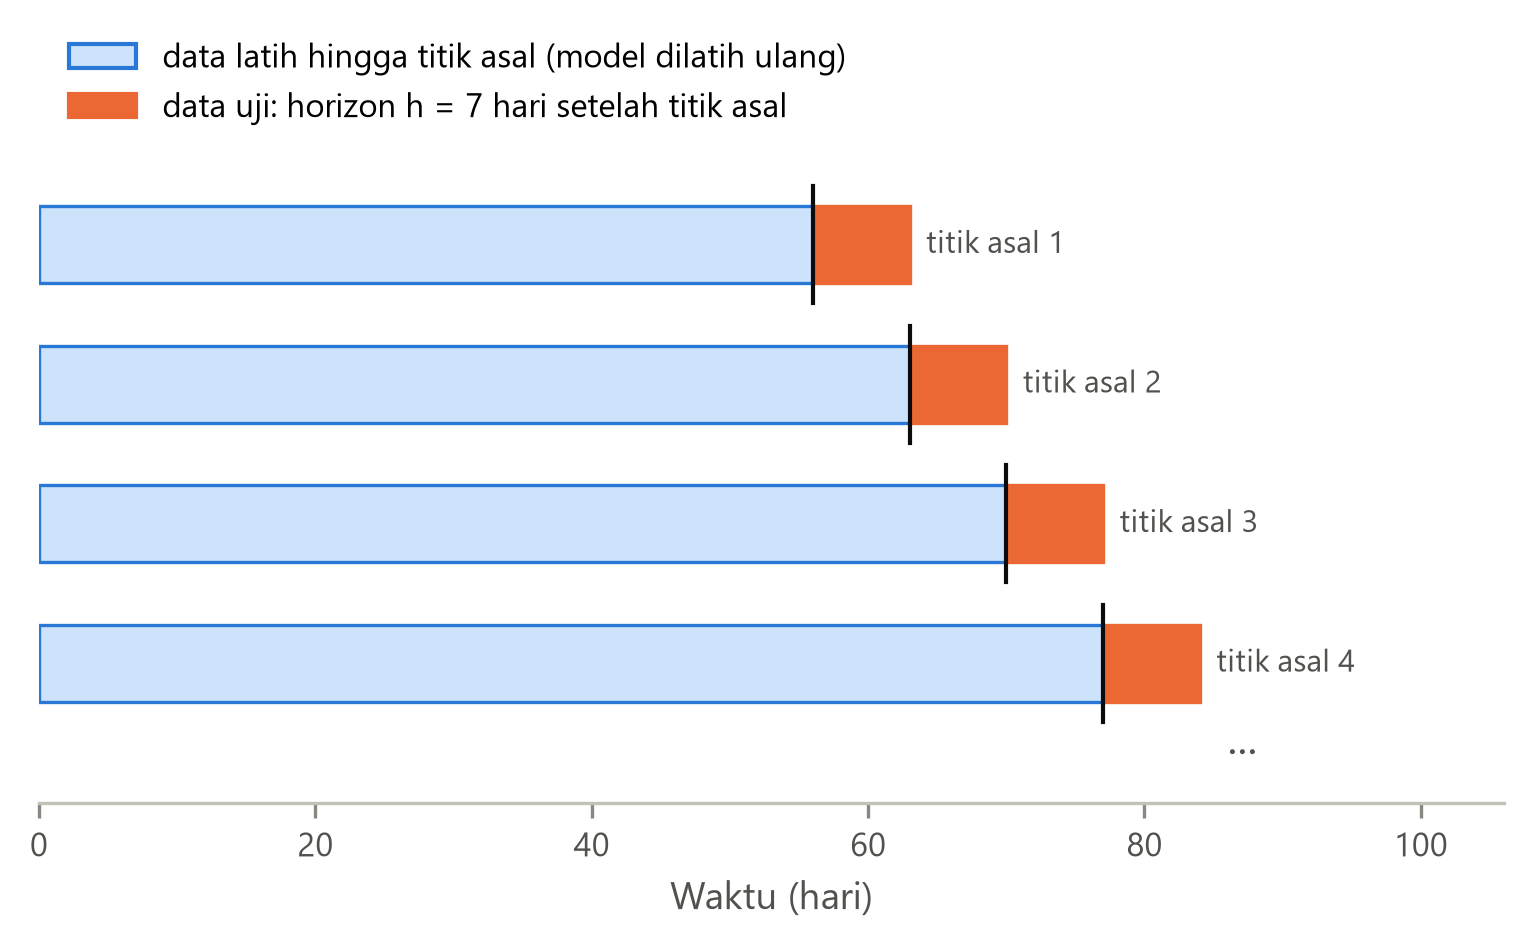
\includegraphics[width=0.78\textwidth]{pic/rolling_origin.png}
\caption{Skema Evaluasi \textit{Rolling Origin}}
\label{fig:rolling-origin}
\end{figure}

%-----------------------------------------------------------------------------%
\subsection{Sistem Pakar dan \texorpdfstring{\textit{Forward Chaining}}{Forward Chaining}}
\label{subsec:sistem-pakar}

Sistem pakar adalah sistem berbasis pengetahuan yang dapat mendukung, dan kadang menggantikan, pakar dalam mengambil keputusan. Komponen penyusunnya adalah basis pengetahuan, mesin inferensi, dan antarmuka pengguna, dan validasinya penting karena banyak sistem pakar dalam literatur tidak divalidasi \citep*{saibene2021expert}. Basis pengetahuan menyimpan pengetahuan domain sebagai aturan produksi JIKA--MAKA (\textit{IF--THEN}), mesin inferensi menerapkan aturan pada fakta untuk menarik kesimpulan, dan antarmuka menerima masukan serta menampilkan kesimpulan. \textit{Backward chaining} menalar dari tujuan menuju fakta pendukungnya, sedangkan \textit{forward chaining} menalar dari fakta yang diketahui: setiap aturan yang seluruh premisnya terpenuhi dijalankan (\textit{fired}), konklusinya ditambahkan ke memori kerja sebagai fakta baru, dan proses diulang hingga tidak ada fakta baru; kedua metode dibahas dalam buku ajar \citet*{russell2021artificial}. Algoritma~\ref{alg:forward-chaining}, yang disusun penulis, menuliskan \textit{forward chaining} dengan jejak aturan sebagaimana dipakai pada penelitian ini. Metode ini cocok untuk diagnosis seduhan karena masukannya berupa data yang dikumpulkan lebih dahulu, yaitu hasil pengukuran dan keluhan rasa, dan sistem perlu menurunkan semua kesimpulan yang relevan dari data itu.

\begin{algorithm}[htbp]
\caption{\textit{Forward Chaining} dengan Jejak Aturan}
\label{alg:forward-chaining}
\begin{algorithmic}[1]
\Require himpunan fakta awal $F$; himpunan aturan $\mathcal{R}$, setiap aturan $r$ memiliki premis $P_r$, konklusi $C_r$, dan prioritas
\Ensure himpunan fakta akhir $F$ dan jejak aturan terpicu $J$
\State $J \gets$ daftar kosong
\Repeat
  \State $\mathit{baru} \gets \mathit{salah}$
  \For{setiap aturan $r \in \mathcal{R}$ yang belum terpicu, urut menurut prioritas}
    \If{$P_r \subseteq F$}
      \State $F \gets F \cup C_r$; tambahkan $r$ beserta premis yang memenuhinya ke $J$
      \State $\mathit{baru} \gets \mathit{benar}$
    \EndIf
  \EndFor
\Until{$\mathit{baru} = \mathit{salah}$}
\State \Return $F$, $J$
\end{algorithmic}
\end{algorithm}

Takar menyediakan fasilitas penjelasan (\textit{explanation facility}) berupa jejak aturan yang terpicu beserta premis yang memenuhinya, sehingga barista dapat melihat alasan di balik setiap saran; pola serupa dipakai sistem pakar diet pasien GERD di Indonesia yang memakai \textit{forward chaining} dengan faktor kepastian untuk menghasilkan rekomendasi \textit{top}-$N$ disertai jejak alasan (\textit{reason traces}) dari aturan yang bersumber dari pedoman klinis \citep*{maulia2026rulebased}. Basis pengetahuan Takar disusun dari literatur penyeduhan pada Subbab~\ref{subsec:penyeduhan} dan dari standar resep yang tersimpan di aplikasi, yaitu parameter resep arahan seperti rasio 1:15 dan waktu seduh V60 serta asumsi yang didokumentasikan untuk resep tambahan. Setiap aturan menyimpan sumbernya, yaitu rujukan pustaka atau standar resep, sehingga penjelasan kepada barista dapat ditelusuri. Fakta masukannya berupa metode seduh, dosis, dan massa air atau minuman, ditambah TDS, waktu kontak, suhu air, dan keluhan rasa bila tersedia; fakta turunannya berupa rasio seduh, EY, dan zona pada bagan kendali seduh; dan konklusinya berupa rekomendasi seperti mengubah gilingan, rasio atau dosis, dan waktu kontak, dengan perubahan suhu air sebagai prioritas terendah sesuai temuan \citet*{batali2020brew}. Aturan lengkapnya disajikan pada Tabel~\ref{tab:aturan-pakar} di Bab~\ref{bab:metode}. Aturan tegas (\textit{crisp}) memiliki keterbatasan, karena batas zona bagan kendali bukan batas preferensi yang universal \citep*{cotter2020consumer} dan arah koreksi gilingan tidak selalu monoton \citep*{lee2023uneven}. Logika \textit{fuzzy}, yang pernah dipakai untuk menentukan tekanan piston mesin kopi \citep*{hadianto2023design}, dapat memodelkan batas yang tidak tegas, sedangkan pembelajaran penguatan dapat belajar dari data seduhan \citep*{bramantoro2025optimization} tetapi memerlukan data berlabel yang tidak tersedia pada penelitian ini. Sistem pakar Takar diuji dengan tabel keputusan yang mencakup setiap aturan dan divalidasi secara eksternal terhadap data konsumen UC Davis \citep*{ristenpart2023consumer} dan resep seduh \citet*{batali2020brew}.

%-----------------------------------------------------------------------------%
\subsection{Model Bahasa Lokal, Pencarian Dokumen, dan \texorpdfstring{\textit{Retrieval-Augmented Generation}}{Retrieval-Augmented Generation}}
\label{subsec:llm-rag}

Model bahasa besar (\textit{large language model}, LLM) menghasilkan teks berdasarkan pola yang dipelajari selama pelatihan, tetapi pengetahuan di dalam parameternya tidak selalu dapat diakses atau dimanipulasi secara tepat dan sumber suatu pernyataan sulit ditelusuri \citep{lewis2020retrievalaugmented}. Survei tentang halusinasi mendefinisikan keluaran yang bertentangan dengan sumber sebagai halusinasi intrinsik dan keluaran yang tidak dapat diverifikasi dari sumber sebagai halusinasi ekstrinsik \citep{ji2023survey}. Pada aplikasi bar kopi, angka resep, stok, dan waktu seduh dapat berubah ketika standar kedai diperbarui. Karena itu, jawaban model yang terdengar meyakinkan belum cukup: sumbernya perlu ditampilkan, dan angka operasional perlu diperoleh dari fungsi aplikasi yang menyimpan data terbaru.

\textit{Retrieval-augmented generation} (RAG) menggabungkan model bahasa dengan pengetahuan eksternal yang dicari pada waktu menjawab. Rancangan awal \citet{lewis2020retrievalaugmented} memakai memori nonparametrik berupa indeks vektor Wikipedia dan pencari neural; dengan demikian RAG tidak identik dengan satu jenis pencarian tertentu. Survei \citet{fan2024survey} membedakan pencari \textit{sparse} dan \textit{dense}, serta menerangkan bentuk sederhana yang menambahkan bagian dokumen hasil pencarian ke masukan model saat inferensi. Takar menerapkan bentuk ini pada resep, SOP, aturan koreksi seduh, dan glosarium internal. Potongan yang ditemukan membawa pengenal serta tautan sumber agar jawaban dapat diperiksa oleh barista; perubahan dokumen dapat masuk ke korpus tanpa melatih ulang bobot model.

Pencarian korpus Takar memakai BM25, metode pemeringkatan dokumen dalam kerangka relevansi probabilistik \citep*{robertson2009probabilistic}. Skor BM25 memperhatikan frekuensi kata kueri di suatu dokumen, kelangkaan kata itu di korpus, dan panjang dokumen relatif terhadap rata-rata korpus. Parameter $k_1$ mengatur kejenuhan pengaruh frekuensi, sedangkan $b$ mengatur normalisasi panjang dokumen; pemilihan nilainya tetap perlu diuji pada korpus yang dipakai, sebab sumbernya tidak memberi nilai terbaik yang berlaku universal \citep*{robertson2009probabilistic}. Pencarian leksikal ini transparan dan dapat berjalan sepenuhnya lokal, tetapi perbedaan istilah pengguna dan dokumen dapat menurunkan temuan. Normalisasi aksen, kata umum, dan sinonim kecil bahasa Indonesia--Inggris dipakai agar pertanyaan seperti ``susu'' dan istilah \textit{milk} dapat menjangkau potongan yang sama. Kualitasnya dinilai dengan posisi potongan acuan dalam daftar hasil, antara lain \textit{Recall}@1/3/5 dan \textit{mean reciprocal rank} (MRR).

Dokumen yang ditemukan saja tidak cukup untuk pertanyaan yang membutuhkan perhitungan. \citet{schick2023toolformer} menunjukkan bahwa model bahasa dapat memilih API, argumen, dan pemakaian hasilnya, terutama untuk tugas seperti aritmetika atau pencarian fakta yang sulit ditangani model bahasa sendiri. Arsitektur \textit{function calling} lokal memungkinkan model mengirim nama fungsi dan argumen terstruktur, aplikasi menjalankan fungsi itu, lalu hasilnya dikembalikan sebagai konteks jawaban \citep*{ollama2026ollama}. Penelitian perencanaan pemanggilan fungsi dari bahasa Indonesia pada pencarian restoran menunjukkan potensi keluaran JSON terstruktur, tetapi juga mencatat kesulitan menyusun semua parameter dengan tepat dalam satu sesi \citep*{mauludin2026large}. Dalam Takar, keluaran alat takaran, diagnosis, stok, dan pasangan menu diperiksa terhadap layanan asli; fungsi tidak diberi hak mengubah inventaris melalui chat.

Model dipilih agar layanan dapat dijalankan tanpa API eksternal. Laporan teknis \citet*{gemmateam2026gemma4} menyajikan Gemma 4 sebagai keluarga model berbobot terbuka dengan varian berukuran kecil E2B dan E4B serta dukungan format pemanggilan fungsi. Ollama menyediakan layanan lokal untuk menjalankan model dan API percakapan dengan definisi alat \citep*{ollama2026ollama}. Menjalankan inferensi di komputer kedai menghilangkan kebutuhan mengirim pertanyaan ke layanan model awan, tetapi bukan jaminan kerahasiaan otomatis: akses server dan penyimpanan log tetap harus dikelola. Kinerja bahasa Indonesia juga tidak dapat diasumsikan dari tolok ukur bahasa Inggris; \citet*{koto2023large} menunjukkan pentingnya evaluasi tersendiri pada bahasa dan konteks Indonesia.

RAG mengurangi risiko jawaban tanpa dasar, tetapi tidak menghilangkannya. \citet*{chen2024benchmarking} menilai kemampuan menolak pertanyaan yang tidak dijawab dokumen sebagai aspek mendasar RAG dan menemukan model yang diuji masih kesulitan pada penolakan, integrasi informasi, serta dokumen yang menyesatkan. \citet*{es2024ragas} memisahkan mutu pencarian konteks, kesetiaan jawaban terhadap konteks, dan relevansi jawaban dalam evaluasi RAG. Karena itu, penelitian ini membandingkan pencarian saja, LLM tanpa dokumen, LLM dengan RAG, serta LLM dengan RAG dan alat pada pertanyaan resep, prosedur, perhitungan, diagnosis, stok, dan pertanyaan di luar cakupan. Angka yang tidak terdapat dalam pertanyaan, dokumen yang diberikan, atau hasil alat dihitung sebagai angka tanpa dasar menurut definisi operasional penelitian; ukuran ini tidak menggantikan pemeriksaan manusia atas benar-salahnya keseluruhan jawaban.

%-----------------------------------------------------------------------------%
\subsection{Evaluasi Sistem Rekomendasi}
\label{subsec:evaluasi-rekomendasi}

Evaluasi sistem rekomendasi memerlukan keputusan tentang tujuan, metode, data, dan metrik, dan sering memerlukan beberapa sudut pandang \citep*{zangerle2022evaluating}. Penelitian ini memakai evaluasi luring (\textit{offline}) pada transaksi historis untuk ketepatan rekomendasi dan UAT untuk penerimaan pengguna. Untuk tugas \textit{top}-$N$, yaitu menampilkan daftar rekomendasi teratas tanpa nilai prediksi, metrik berbasis galat seperti RMSE kurang cocok, dan kinerja lebih tepat diukur dengan metrik akurasi seperti \textit{precision} dan \textit{recall} \citep*{cremonesi2010performance}. Protokolnya mengadaptasi \citet*{deshpande2004itembased}, yang menyembunyikan satu \textit{item} acak dari setiap pengguna, memakai \textit{item} sisanya sebagai keranjang, dan menghitung \textit{hit} bila \textit{item} yang disembunyikan muncul di daftar rekomendasi. Penelitian ini menyembunyikan setiap \textit{item} keranjang uji secara bergantian (\textit{leave-one-out}), sehingga keranjang berisi $b$ menu berbeda menghasilkan $b$ kueri; adaptasi ini adalah rancangan penulis. \textit{Hit rate} dan \textit{precision} pada $K$ rekomendasi teratas adalah \citep*{deshpande2004itembased, cremonesi2010performance}
\begin{equation}
\mathrm{HR@}K = \frac{\#\mathrm{hit}}{n} = \frac{1}{n}\sum_{q=1}^{n} \mathbf{1}\left[\, i_q \in L_K(q) \,\right],
\label{eq:hr}
\end{equation}
\begin{equation}
\mathrm{P@}K = \frac{\#\mathrm{hit}}{K \cdot |T|} = \frac{\mathrm{HR@}K}{K},
\label{eq:precision-k}
\end{equation}
dengan $n$ jumlah kueri uji, $i_q$ \textit{item} yang disembunyikan pada kueri $q$, $L_K(q)$ daftar $K$ rekomendasi teratas, $\mathbf{1}[\cdot]$ fungsi indikator, dan $|T|$ jumlah kasus uji. Persamaan~\eqref{eq:precision-k} berlaku bila setiap kueri memiliki tepat satu \textit{item} relevan; secara umum, \textit{precision}@$K$ adalah proporsi \textit{item} relevan di antara $K$ rekomendasi \citep*{zangerle2022evaluating}, sehingga di sini P@5 paling besar 0,2 secara definisi.

HR@$K$ tidak membedakan \textit{hit} di posisi pertama dan terakhir, sedangkan \textit{mean reciprocal rank} (MRR@$K$) memberi bobot lebih besar pada \textit{hit} di posisi awal; untuk satu \textit{item} tersembunyi per kueri, MRR@$K$ sama dengan \textit{average reciprocal hit-rank} dari \citet*{deshpande2004itembased}. Cakupan katalog (\textit{catalogue coverage}) mengukur seberapa banyak \textit{item} yang pernah muncul dalam daftar rekomendasi \citep*{zangerle2022evaluating, latifi2021sessionaware}:
\begin{equation}
\mathrm{MRR@}K = \frac{1}{n}\sum_{i=1}^{h} \frac{1}{p_i},
\label{eq:mrr}
\end{equation}
\begin{equation}
\mathrm{Cov}_{\mathrm{katalog}} = \frac{\left|\bigcup_{q=1}^{n} L_K(q)\right|}{|I|},
\label{eq:coverage}
\end{equation}
dengan $h$ jumlah \textit{hit} dalam daftar \textit{top}-$K$, $p_i$ peringkat \textit{hit} ke-$i$ (kueri tanpa \textit{hit} menyumbang nol), dan $I$ himpunan seluruh \textit{item} katalog; notasi Persamaan~\eqref{eq:coverage} dituliskan penulis dari definisi verbal sumber. Sistem yang hanya merekomendasikan beberapa menu terpopuler dapat memiliki HR tinggi tetapi cakupan rendah. Penelitian ini juga melaporkan cakupan kueri, yaitu proporsi kueri yang memicu sedikitnya satu aturan asosiasi, sebagai ukuran yang didefinisikan penulis. Metode yang diusulkan juga harus dibandingkan dengan pembanding sederhana, karena algoritma nonpersonal yang naif dapat mengungguli sebagian pendekatan rekomendasi yang umum \citep*{cremonesi2010performance} dan 11 dari 12 pendekatan rekomendasi neural yang dapat direproduksi dapat dikalahkan metode sederhana \citep*{ferraridacrema2021troubling}. Karena itu, FP-Growth dibandingkan dengan pembanding popularitas dan kemunculan bersama (\textit{co-occurrence}), yaitu peringkat kandidat menurut peluang bersyarat kemunculannya bersama menu di keranjang.

Pembagian data harus mengikuti urutan waktu. Kebocoran data (\textit{data leakage}) terjadi ketika informasi yang tidak tersedia pada saat prediksi ikut dipakai dalam pelatihan atau pemilihan model. Pembagian yang mengabaikan garis waktu global membuat model rekomendasi belajar dari interaksi yang belum terjadi, sehingga model dapat merekomendasikan \textit{item} masa depan dan urutan peringkat model menjadi tidak dapat diprediksi \citep*{ji2023critical}. \citet*{kapoor2023leakage} menemukan kebocoran di 17 bidang ilmu yang memengaruhi 294 makalah dan menyusun taksonomi delapan jenis kebocoran, termasuk kebocoran temporal. Penelitian ini karenanya menambang aturan dari periode awal dan mengujinya pada periode sesudahnya, memilih ambang parameter pada potongan validasi di ujung periode latih, dan melatih model peramalan hanya dengan data hingga titik asalnya.

Perbedaan antarmetode juga perlu disertai ketidakpastiannya. \textit{Bootstrap} diperkenalkan \citet*{efron1979bootstrap} sebagai metode umum untuk menaksir distribusi sampling suatu statistik dengan mengambil ulang sampel yang teramati, dan buku ajar \citet*{efron1994introduction} menyajikannya sebagai metode inferensi berbasis komputer, termasuk interval kepercayaan berbasis persentil \textit{bootstrap}. Pada penelitian ini, keranjang uji diambil ulang dengan pengembalian sebanyak $B$ kali; pada setiap replikasi, metrik setiap metode dan selisih berpasangannya dihitung pada keranjang yang sama, lalu batas interval kepercayaan 95\% diambil dari persentil ke-2,5 dan ke-97,5 distribusi replikasi. Unit pengambilan ulangnya adalah keranjang karena kueri dari satu keranjang saling berkaitan, dan H2 dinyatakan didukung bila batas bawah interval selisih HR@5 FP-Growth terhadap popularitas lebih besar dari nol.

%-----------------------------------------------------------------------------%
\subsection{Scrum}
\label{subsec:scrum}

Scrum adalah kerangka kerja ringan yang membantu orang, tim, dan organisasi menghasilkan nilai melalui solusi adaptif untuk masalah yang kompleks; Scrum berlandaskan empirisme, memakai pendekatan iteratif dan inkremental, dan bertumpu pada pilar transparansi, inspeksi, dan adaptasi \citep*{schwaber2020scrum}. \textit{Product Owner} mengurutkan pekerjaan dalam \textit{Product Backlog}, tim mengubah sebagian pekerjaan itu menjadi \textit{Increment} selama satu \textit{Sprint} yang berdurasi paling lama satu bulan, lalu hasilnya diperiksa bersama pemangku kepentingan. \textit{Scrum Guide} menetapkan akuntabilitas \textit{Developers}, \textit{Product Owner}, dan \textit{Scrum Master}; \textit{event} \textit{Sprint Planning}, \textit{Daily Scrum}, \textit{Sprint Review}, dan \textit{Sprint Retrospective}; serta artefak \textit{Product Backlog}, \textit{Sprint Backlog}, dan \textit{Increment} \citep*{schwaber2020scrum}. Kebutuhan dalam \textit{backlog} lazim ditulis sebagai \textit{user story}, yaitu penjelasan informal tentang fitur dari sudut pandang pengguna akhir yang dilengkapi kriteria penerimaan (\textit{acceptance criteria}) untuk memverifikasinya \citep*{ferreira2022towards}; pada penelitian ini, kriteria tersebut menjadi dasar skenario pengujian \textit{black-box} dan UAT. Scrum sering dimodifikasi dalam praktik, dan tinjauan sistematis \citet*{hron2022why} mengidentifikasi sembilan tujuan modifikasinya, antara lain konteks nonstandar. Karena penelitian ini dikerjakan satu mahasiswa, Scrum diterapkan dalam bentuk yang disesuaikan dengan tetap mempertahankan tinjauan hasil bersama pemangku kepentingan dan retrospeksi, sejalan dengan faktor kepedulian terhadap pemangku kepentingan dan perbaikan berkelanjutan pada teori efektivitas tim Scrum \citep*{verwijs2023theory}; rinciannya dibahas pada Subbab~\ref{sec:tahapan}.

%-----------------------------------------------------------------------------%
\subsection{\texorpdfstring{\textit{Unified Modeling Language}}{Unified Modeling Language}}
\label{subsec:uml}

\textit{Unified Modeling Language} (UML) adalah bahasa grafis untuk memvisualisasikan, menspesifikasikan, membangun, dan mendokumentasikan artefak sistem; versi 2.5.1 mendefinisikan notasi diagram kelas, aktivitas, sekuens, dan \textit{use case} \citep*{omg2017unified}. Tinjauan sistematis atas 128 makalah menyebut diagram UML sebagai standar yang diterima untuk menggambarkan model desain berorientasi objek \citep*{koc2021uml}. Penelitian ini memakai diagram \textit{use case} untuk menggambarkan aktor (barista, \textit{head barista}, dan manajer) beserta layanan sistem yang dapat mereka jalankan, diagram aktivitas untuk alur kerja berupa aksi, keputusan, dan partisi tanggung jawab, serta diagram sekuens untuk pesan antarobjek menurut urutan waktu, misalnya antara antarmuka Vue, API FastAPI, layanan penskalaan, dan basis data \citep*{omg2017unified}. Struktur data dimodelkan dengan ERD karena skema basis data menjadi kontrak utama sistem. Diagram-diagram tersebut disajikan pada Subbab~\ref{sec:perancangan-sistem}.

%-----------------------------------------------------------------------------%
\subsection{Pengujian Perangkat Lunak}
\label{subsec:pengujian}

Model kualitas produk ISO/IEC 25010:2023 terdiri atas sembilan karakteristik yang dapat dipakai untuk menetapkan tujuan pengujian dan kriteria penerimaan \citep*{isoiec2023systems}. Penelitian ini memakai tiga kelompok pengujian untuk menjawab RM4: pengujian fungsional \textit{black-box}, pengukuran kinerja, dan uji penerimaan pengguna. Pengujian \textit{black-box} merancang kasus uji dari spesifikasi tanpa melihat struktur internal program, dengan teknik klasik \textit{equivalence partitioning} (EP) dan \textit{boundary value analysis} (BVA) \citep*{myers2012art}. EP membagi ranah masukan menjadi kelas ekuivalen yang valid dan tidak valid dengan anggapan bahwa semua nilai dalam satu kelas diperlakukan sama, sedangkan BVA menguji nilai pada batas antarkelas dan di sekitarnya; pengujian pada batas antarsubranah masukan sangat penting bagi mutu perangkat lunak \citep*{dobslaw2023automated}. Misalnya, masukan tambahan \textit{shot} yang valid pada rentang 0--3 memiliki satu kelas valid dan dua kelas tidak valid, dengan nilai batas $-1$, $0$, $3$, dan $4$. Penggabungan lebih dari satu teknik dianjurkan agar kesalahan yang ditemukan lebih beragam \citep*{siahaan2022elearning}. Pengujian diotomatisasi pada beberapa tingkat: uji unit untuk fungsi seperti aturan penskalaan, uji API untuk kode status dan isi respons setiap \textit{endpoint} termasuk kasus 401, 403, dan 422, serta pengujian \textit{end-to-end} (E2E) yang mengotomatiskan peramban untuk meniru tindakan pengguna dan memvalidasi perilaku keseluruhan aplikasi \citep*{leotta2023challenges}. Penelitian ini memakai pytest \citep{krekel2004pytest} untuk uji unit dan API serta Playwright \citep*{microsoft2026playwright} untuk skenario E2E.

Kinerja diukur dari latensi, yaitu waktu sejak permintaan dikirim hingga respons diterima, yang dilaporkan dengan persentil seperti median (p50) dan persentil ke-95 (p95) karena sebagian kecil permintaan dapat jauh lebih lambat daripada umumnya. Pengukuran waktu bervariasi antarpengulangan, dan pada Google Lighthouse agregasi median dari lima pengujian berturut-turut sangat mengurangi variabilitas \citep*{hericko2021representative}. Ambang ``baik'' Core Web Vitals adalah \textit{Largest Contentful Paint} paling lama 2,5~detik, \textit{Interaction to Next Paint} paling lama 200~milidetik, dan \textit{Cumulative Layout Shift} paling besar 0,1 \citep*{walton2024web}, tetapi ukuran ini kurang prediktif terhadap pengalaman pengguna daripada yang diharapkan \citep*{wehner2023agree}, sehingga perlu dilengkapi evaluasi oleh pengguna. Uji penerimaan pengguna (\textit{user acceptance testing}, UAT) adalah jenis uji penerimaan untuk menentukan apakah pengguna yang dituju menerima sistem \citep*{istqb2026user}; UAT memvalidasi perangkat lunak dalam situasi nyata oleh calon penggunanya, dan pengembangan \textit{agile} menuntut UAT yang sering karena rilisnya kecil dan iteratif \citep*{otaduy2017user}. UAT berbeda dari pengujian \textit{usability}, yang menilai pengalaman pengguna saat berinteraksi dengan produk \citep*{vanesha2024comparison}.

\textit{System Usability Scale} (SUS) adalah skala Likert sepuluh butir yang memberi gambaran global tentang \textit{usability} subjektif; butirnya berselang-seling antara pernyataan positif dan negatif, setiap butir menyumbang 0--4 poin, jumlahnya dikalikan 2,5 sehingga skor berada pada rentang 0--100, dan skor per butir tidak bermakna bila berdiri sendiri \citep*{brooke1996sus}. Skor SUS dihitung dengan (\citealp*{brooke1996sus}; \citealp{hyzy2022system})
\begin{equation}
\mathrm{SUS} = 2{,}5 \left[\sum_{i \in \{1,3,5,7,9\}} (x_i - 1) + \sum_{i \in \{2,4,6,8,10\}} (5 - x_i)\right],
\label{eq:sus}
\end{equation}
dengan $x_i$ posisi jawaban butir ke-$i$ pada skala 1 (sangat tidak setuju) sampai 5 (sangat setuju); butir ganjil bernada positif dan butir genap bernada negatif. SUS adalah kuesioner baku yang paling banyak dipakai untuk menilai \textit{usability} yang dipersepsikan dan terbukti cepat tetapi tidak ``\textit{dirty}'' \citep*{lewis2018system}. Untuk menafsirkan skor, \citet*{bangor2009determining} menambahkan butir peringkat adjektiva pada hampir 1.000 survei SUS; peringkat itu berkorelasi sangat kuat dengan skor SUS ($r = 0{,}822$), dan rerata skor setiap adjektiva disajikan pada Tabel~\ref{tab:sus-adjektiva}, dengan catatan bahwa adjektiva ``OK'' memiliki ragam terbesar. Meta-analisis 117 skor SUS aplikasi kesehatan digital menyimpulkan bahwa rerata acuan 68 dengan simpangan baku 12,5 layak dipakai \citep{hyzy2022system}; penelitian ini memakai acuan tersebut sebagai pembanding umum, dengan catatan bahwa acuan itu divalidasi pada aplikasi kesehatan digital. Hasil UAT dilaporkan setelah UAT dilaksanakan.

\begin{table}[!htb]
\centering
\caption{Rerata Skor SUS per Peringkat Adjektiva}
\label{tab:sus-adjektiva}
{\small
\setstretch{1.0}
\begin{tabular}{@{}lc@{}}
\toprule
\textbf{Peringkat Adjektiva} & \textbf{Rerata Skor SUS} \\
\midrule
\textit{Worst Imaginable} (terburuk yang dapat dibayangkan) & 12,5 \\
\textit{Awful} (sangat buruk) & 20,3 \\
\textit{Poor} (buruk) & 35,7 \\
\textit{OK} (cukup) & 50,9 \\
\textit{Good} (baik) & 71,4 \\
\textit{Excellent} (sangat baik) & 85,5 \\
\textit{Best Imaginable} (terbaik yang dapat dibayangkan) & 90,9 \\
\bottomrule
\end{tabular}}

\vspace{2pt}
{\footnotesize Sumber: \citet*{bangor2009determining}, $n = 959$ survei.}
\end{table}

%=============================================================================%
\section{Penelitian Terkait}
\label{sec:penelitian-terkait}

Penelitian terkait dipilih dengan mengutamakan penelitian terapan tahun 2021--2026 tentang sistem kedai kopi dan usaha makanan dan minuman, terutama di Indonesia, dan dikelompokkan ke dalam lima tema, yaitu sistem informasi operasional, penskalaan dan adaptasi resep, rekomendasi menu dengan aturan asosiasi, peramalan permintaan dan persediaan, serta kecerdasan buatan untuk parameter seduh. Tabel~\ref{tab:penelitian-terkait} membandingkan penelitian yang paling dekat berdasarkan objek, platform, metode, evaluasi, serta hasil dan keterbatasannya. Isi tabel disarikan dari abstrak dan, bila tersedia, dari catatan pembacaan teks lengkap. Informasi yang tidak dinyatakan pada sumber ditulis ``tidak dirinci''.

\textbf{Sistem informasi operasional.} Penelitian Indonesia pada tema ini umumnya membangun sistem web untuk satu kelompok kebutuhan. Contohnya adalah inventaris kopi di sebuah kedai di Sukabumi \citep*{alifadillah2023web}, stok bahan baku dengan Laravel dan MySQL beserta log aktivitas di sebuah kafe di Pontianak \citep*{abdur2026sistem}, \textit{safety stock} dan ROP dengan notifikasi stok minimum di Kava Coffee Shop, Kudus \citep*{taufiq2025implementation}, kasir, stok, dan laporan keuangan di Natta Coffee \citep*{rusmara2025pengembangan}, harga pokok produksi rumah makan dari komposisi resep \citep*{kartono2025perancangan}, kasir PWA untuk UMKM \citep*{prayudha2024rancang}, serta digitalisasi SOP perusahaan logistik dengan RBAC tiga peran \citep*{shabrina2026sistem}. Arsitektur PWA luring-dahulu dengan \textit{service worker}, antrean IndexedDB, dan \textit{background sync} mempertahankan seluruh transaksi kasir yang diantrekan selama gangguan jaringan pada kondisi yang diuji, walaupun konsistensi persediaan masih perlu divalidasi \citep*{nugraha2026implementation}. Sejauh yang dilaporkan, tidak satu pun sistem tersebut menggabungkan resep standar, penskalaan takaran, dan pemotongan stok otomatis dari produksi.

\textbf{Penskalaan dan adaptasi resep.} \citet*{benita2026web} membangun platform web yang menghitung ulang takaran masakan rumah tangga sesuai jumlah porsi dengan penggantian bahan, pengaturan tingkat pedas, dan asisten memasak berbasis AI, tetapi abstraknya hanya menyajikan prototipe dan rencana evaluasi. \citet{choi2023kitchenscale} memprediksi kuantitas dan satuan bahan dari konteks resep dengan model bahasa praterlatih, sedangkan \citet*{moralesgarzon2025service} mengadaptasi resep melalui penggantian bahan sesuai preferensi, tujuan kesehatan dan keberlanjutan, serta alergi pengguna. Sejauh yang tampak dari abstraknya, tidak ada yang memodelkan batasan bar kopi atau membandingkan hasilnya dengan penskalaan linier.

\textbf{Rekomendasi menu dengan aturan asosiasi.} FP-Growth telah diterapkan pada data penjualan Cascara Coffee \citep*{fadillah2021data}, Cafe Over Limit \citep*{hasan2023utilization}, dan Kedai Kopi Raja Palembang \citep*{pratama2025food}, serta pada \textit{dataset} Bread Basket \citep*{sihombing2026analisis}, yaitu transaksi nyata sebuah toko roti di Edinburgh \citep*{mittal2020bread} yang juga dipakai pada validasi eksternal penelitian ini dengan catatan lisensinya tidak jelas. Apriori dipakai untuk perencanaan pasokan kopi di Setuju Coffee \citep*{nasution2025application} dan rekomendasi menu aplikasi pemesanan dengan 200 transaksi simulasi \citep*{yudanto2025penerapan}, sedangkan sistem rekomendasi menu kedai kopi yang dibangun \citet*{rahmatika2025sistem} hanya menghitung \textit{support} pasangan menu. Sistem yang paling dekat dengan Takar adalah sistem rekomendasi menu katering industri yang dibangun \citet*{pratama2026automatic}; sistem tersebut memadukan penyaringan menu berdasarkan stok dan anggaran, K-Means, dan Apriori serta memotong stok bahan secara otomatis. Sejauh yang tampak dari abstrak dan catatan teks lengkap yang tersedia, penelitian-penelitian ini menilai aturan pada seluruh data, umumnya dengan \textit{support}, \textit{confidence}, dan \textit{lift} atau, pada \citet*{rahmatika2025sistem}, hanya dengan \textit{support}, tanpa menguji ketepatan rekomendasi pada transaksi periode berikutnya atau membandingkannya dengan pembanding sederhana.

\textbf{Peramalan permintaan dan persediaan.} Pada kedai kopi, ARIMA memberi galat terendah dibandingkan rata-rata bergerak dan SARIMA untuk penjualan harian satu produk \citep*{azzahra2025forecasting} dan juga terbaik dibandingkan Prophet dan LSTM setelah penalaan \citep*{pattisealnno2026comparative}. \citet*{windrasari2025predictive} memprediksi penjualan kedai kopi dengan \textit{random forest} tanpa hasil pembanding; karakteristik datanya, yaitu 149.116 transaksi Januari--Juni 2023 dari tiga gerai bernama Astoria, Hell's Kitchen, dan Lower Manhattan, sama dengan \textit{dataset} Maven Coffee Shop Sales yang dinyatakan penerbitnya sebagai data kedai kopi fiktif \citep*{mavenanalytics2023coffee}, walaupun makalah tersebut tidak menyebut sumber datanya. Pada sisi persediaan, \citet*{lauren2026optimizing} menggabungkan ramalan DR-ARMA dengan stok pengaman berbasis galat untuk UMKM kuliner, \citet*{piewthongngam2026aienabled} mengubah ramalan LightGBM menjadi kebutuhan bahan melalui rasio pemakaian historis, dan \citet*{nurhalizapratiwi2025analisis} menerapkan EOQ, \textit{safety stock}, dan ROP pada bahan kopi susu. Sejauh penelusuran penulis, belum ada penelitian kedai kopi yang menurunkan kebutuhan bahan dari resep standar yang juga dipakai untuk memotong stok, lalu menguji kebijakan \textit{restock}-nya terhadap ROP statis dalam simulasi.

\textbf{Kecerdasan buatan untuk parameter seduh.} \citet*{bramantoro2025optimization} dan \citet*{jeffery2025optimizing} mengoptimalkan variabel \textit{pour over} dengan pembelajaran penguatan; kedua pendekatan ini menghasilkan model yang dipelajari, bukan aturan eksplisit yang dapat ditelusuri ke sumber pustaka, dan pendekatan pertama memerlukan data seduhan berlabel dari barista dan penyeduh rumahan. \citet*{apiletti2020correlating} menambang aturan asosiasi yang dapat dibaca manusia dan mengaitkan mutu espreso dengan pengaturan gilingan, waktu ekstraksi, dan dosis, tetapi aturan tersebut ditambang dari data seduhan mesin espreso profesional, bukan disusun dari literatur penyeduhan. Sistem pakar \textit{forward chaining} dipakai untuk memilih biji kopi pascasangrai \citep*{anggraeni2024sistem} dan mendiagnosis kerusakan mesin espreso \citep*{rizal2024sistem}. Sejauh penelusuran penulis, sistem pakar kopi yang ditemukan belum menyentuh koreksi parameter seduh berbasis bagan kendali seduh.

\begin{landscape}
{\scriptsize
\setstretch{1.0}
\setlength{\tabcolsep}{3pt}
\renewcommand{\arraystretch}{1.1}
\begin{longtable}{@{}>{\raggedright\arraybackslash}p{2.8cm}>{\raggedright\arraybackslash}p{3.1cm}>{\raggedright\arraybackslash}p{3.0cm}>{\raggedright\arraybackslash}p{4.4cm}>{\raggedright\arraybackslash}p{3.6cm}>{\raggedright\arraybackslash}p{5.6cm}@{}}
\caption{Perbandingan Penelitian Terkait}
\label{tab:penelitian-terkait} \\
\toprule
\textbf{Peneliti (Tahun)} & \textbf{Objek/Konteks} & \textbf{Platform/Teknologi} & \textbf{Metode/Fitur} & \textbf{Evaluasi} & \textbf{Hasil/Keterbatasan} \\
\midrule
\endfirsthead
\multicolumn{6}{@{}l}{\small\textit{Tabel~\ref{tab:penelitian-terkait} (lanjutan)}} \\
\toprule
\textbf{Peneliti (Tahun)} & \textbf{Objek/Konteks} & \textbf{Platform/Teknologi} & \textbf{Metode/Fitur} & \textbf{Evaluasi} & \textbf{Hasil/Keterbatasan} \\
\midrule
\endhead
\midrule
\multicolumn{6}{@{}r}{\small\textit{bersambung ke halaman berikutnya}} \\
\endfoot
\bottomrule
\endlastfoot
\citet*{alifadillah2023web} & Kedai kopi di Sukabumi & Web, MySQL (XAMPP) & Aplikasi inventaris kopi & Wawancara, observasi, uji sistem & Perbaikan dilaporkan kualitatif; menyarankan analitik prediktif \\
\addlinespace
\citet*{abdur2026sistem} & Kafe di Pontianak & Laravel, MySQL; \textit{Waterfall} & Stok bahan baku, \textit{preset} barang, log aktivitas & \textit{Black-box}; UAT 12 responden & UAT sekitar 94\%; pemotongan stok dari resep tidak dirinci \\
\addlinespace
\citet*{taufiq2025implementation} & Kava Coffee Shop, Kudus & Web; \textit{Waterfall} & \textit{Safety stock}, ROP, notifikasi stok minimum, pelacakan kedaluwarsa & \textit{Black-box} & Keberhasilan uji 100\%; tanpa peramalan dan BOM resep \\
\addlinespace
\citet*{rusmara2025pengembangan} & Natta Coffee & Laravel (MVC); RAD (\textit{Rapid Application Development}) & Kasir, stok, laporan keuangan & \textit{Black-box} & Klaim perbaikan tanpa pengukuran waktu atau UAT \\
\addlinespace
\citet*{prayudha2024rancang} & UMKM & PWA, Laravel & Kasir (\textit{point of sale}) & \textit{Black-box} 83 skenario, UAT, Lighthouse & Semua skenario lolos; UAT 544 dari 600; hanya transaksi \\
\addlinespace
\citet*{nugraha2026implementation} & Dasbor kasir Mangkasir & Next.js, PWA luring-dahulu & \textit{Service worker}, antrean IndexedDB, \textit{background sync} & \textit{Black-box}, uji sinkronisasi & Transaksi antrean terjaga; konsistensi persediaan belum divalidasi \\
\addlinespace
\citet*{kartono2025perancangan} & UMKM kuliner, Pontianak & Web; RAD & Harga pokok produksi berbasis resep & \textit{Black-box}, SUS & SUS 85; pengelolaan stok dan penyajian tidak dirinci \\
\addlinespace
\citet*{benita2026web} & Masakan rumah tangga & React, Node.js, PostgreSQL & Penskalaan per porsi, penggantian bahan, asisten AI & Rencana evaluasi & Prototipe tanpa hasil pada abstrak; batasan bar tidak dirinci \\
\addlinespace
\citet*{fadillah2021data} & Cascara Coffee & Tidak dirinci & FP-Growth untuk \textit{cross-selling} dan \textit{up-selling} & \textit{Lift} & \textit{Lift} tertinggi 2,789 (sebagaimana tercetak); uji pada periode berikutnya tidak dirinci \\
\addlinespace
\citet*{hasan2023utilization} & Cafe Over Limit & Tidak dirinci & FP-Growth (\textit{support} 10\%, \textit{confidence} 50\%) & \textit{Lift} & Dua dari tiga aturan (\textit{lift} 1,15) dinilai sah \\
\addlinespace
\citet*{pratama2025food} & Kedai Kopi Raja Palembang & Python; prototipe & FP-Growth dalam tahapan KDD & \textit{Lift} & 24 aturan; lima aturan ber-\textit{lift} tertinggi menjadi paket menu \\
\addlinespace
\citet*{sihombing2026analisis} & \textit{Dataset} Bread Basket (toko roti, Edinburgh) & RapidMiner & FP-Growth sebagai dasar rekomendasi kasir & \textit{Support}, \textit{confidence}, \textit{lift} & Hanya Cake $\rightarrow$ Coffee berasosiasi positif (\textit{lift} 1,102); analisis luring \\
\addlinespace
\citet*{rahmatika2025sistem} & Kedai kopi (pemesanan) & Laravel & Rekomendasi dari \textit{support} pasangan menu & \textit{Black-box}; SUS 20 responden & SUS 75,7; tanpa \textit{confidence} dan \textit{lift} \\
\addlinespace
\citet*{pratama2026automatic} & Katering industri, Sidoarjo & Laravel 11, MySQL, Python (scikit-learn, MLxtend) & Penyaringan stok dan anggaran, K-Means, Apriori, pemotongan stok otomatis & \textit{Silhouette}, statistik aturan, \textit{black-box} 47 kasus & 83 aturan; uji ketepatan rekomendasi pada data uji tidak dirinci \\
\addlinespace
\citet*{windrasari2025predictive} & Penjualan kedai kopi (data sama dengan \textit{dataset} Maven) & Tidak dirinci & \textit{Random forest} & Validasi silang lima lipatan, MSE & MSE rata-rata 80,97; tanpa pembanding \\
\addlinespace
\citet*{azzahra2025forecasting} & Penjualan harian satu produk & Tidak dirinci & Rata-rata bergerak, ARIMA, SARIMA & MAE, RMSE & ARIMA terbaik; SARIMA lemah karena pola musiman lemah \\
\addlinespace
\citet*{pattisealnno2026comparative} & Penjualan kedai kopi & Tidak dirinci & ARIMA, Prophet, LSTM & MAE, RMSE, MAPE & ARIMA terbaik setelah penalaan; LSTM \textit{overfitting}; pembanding naif tidak dirinci \\
\addlinespace
\citet*{lauren2026optimizing} & UMKM kuliner di Indonesia & Sistem desktop & DR-ARMA, stok pengaman berbasis galat & MAPE, tingkat layanan & MAPE 24,64\% (SMA 42,70\%, naif 24,99\%) pada data dengan lebih dari 30\% hari tanpa penjualan, tanpa rincian penanganan nilai nol; pemakaian resep tidak dirinci \\
\addlinespace
\citet*{piewthongngam2026aienabled} & Restoran prasmanan, Thailand & LightGBM, Optuna & Ramalan ke kebutuhan bahan via rasio pemakaian; segmentasi VVC & Validasi \textit{walk-forward}; biaya bahan rusak & Biaya bahan rusak turun rata-rata 19,4\%; bukan BOM resep \\
\addlinespace
\citet*{bramantoro2025optimization} & Ujala Cafe \& Roastery, Cianjur & Tidak dirinci & Pembelajaran penguatan untuk variabel \textit{pour over} & Akurasi, F1 & Akurasi 90,00\%; data praktisi sedikit; tanpa aturan eksplisit \\
\addlinespace
\citet*{anggraeni2024sistem} & Pemilihan biji kopi pascasangrai & Tidak dirinci & Sistem pakar \textit{forward chaining} & UAT & 90,41\% (antarmuka), 86,87\% (kegunaan) \\
\addlinespace
Penelitian ini & Bar kedai kopi (resep arahan); data sampel fiktif IBM dan Maven; data nyata Bread Basket, ihelon, UC Davis & FastAPI, Vue.js, SQLite; pandas, scikit-learn, statsmodels, mlxtend & Resep standar, SOP, penskalaan berbasis batasan, buku besar stok, FP-Growth, peramalan dan \textit{restock}, sistem pakar & Pembanding linier; pembagian berbasis waktu dan \textit{bootstrap}; \textit{rolling origin}; simulasi; \textit{black-box}, latensi, UAT & Dilaporkan pada Bab~\ref{bab:hasil} \\
\end{longtable}
}
\end{landscape}

Tabel~\ref{tab:penelitian-terkait} memperlihatkan tiga pola. Pertama, sistem informasi kedai kopi dan usaha kuliner umumnya menangani satu fungsi, yaitu stok, kasir, atau biaya, dan dievaluasi dengan pengujian \textit{black-box} serta UAT atau SUS, sedangkan digitalisasi SOP yang ditemukan berasal dari perusahaan logistik. Kedua, penelitian AI pada kedai kopi umumnya berupa analisis data yang berdiri sendiri: aturan asosiasi dinilai pada seluruh data, dan model peramalan tidak selalu dibandingkan dengan pembanding sederhana atau diuji dengan pembagian berbasis waktu. Ketiga, penelitian yang paling dekat dengan Takar menggabungkan sebagian komponen, yaitu rekomendasi menu dengan batasan stok dan pemotongan stok otomatis pada katering \citep*{pratama2026automatic}, ramalan yang diubah menjadi kebutuhan bahan melalui rasio historis \citep*{piewthongngam2026aienabled}, atau ramalan dengan stok pengaman berbasis galat \citep*{lauren2026optimizing}, tetapi tidak dalam konteks bar kopi dengan resep standar dan batasan penyajiannya.

Dari pola-pola tersebut, kesenjangan yang diisi penelitian ini dapat dirumuskan sebagai berikut. Sejauh penelusuran penulis, belum ditemukan penelitian yang mengintegrasikan dalam satu aplikasi web untuk bar kopi (1) resep standar yang menyimpan parameter seduh, SOP, dan BOM-nya; (2) penskalaan takaran berbasis batasan yang menjaga \textit{shot} utuh, kapasitas cangkir, dan rasio seduh, lalu dibandingkan secara kuantitatif dengan penskalaan linier; (3) buku besar persediaan yang dipotong otomatis dari produksi melalui BOM resep; dan (4) rekomendasi AI untuk pasangan menu, \textit{restock} berbasis peramalan, dan koreksi parameter seduh yang dievaluasi, baik pada data sampel fiktif (IBM dan Maven) maupun pada data nyata (Bread Basket, ihelon, dan data konsumen UC Davis), dengan pembanding sederhana dan pembagian data berbasis waktu bagi modul berbasis data serta tabel keputusan bagi sistem pakar. Penelitian ini tidak mengklaim kebaruan algoritmik yang mutlak, karena FP-Growth, Holt-Winters, \textit{gradient boosting}, kebijakan ROP dan \textit{order-up-to}, serta \textit{forward chaining} adalah metode yang sudah mapan. Kontribusinya terletak pada integrasi komponen-komponen tersebut di sekitar resep standar kedai kopi dan pada evaluasi yang terkendali serta jujur terhadap sifat datanya.

%=============================================================================%
\section{Kerangka Pemikiran}
\label{sec:kerangka-pemikiran}

Kerangka pemikiran penelitian ini disusun dari masalah operasional pada arahan penelitian, teori pada Subbab~\ref{sec:landasan-teori}, dan kesenjangan pada Subbab~\ref{sec:penelitian-terkait}. Gambar~\ref{fig:kerangka-pemikiran} merangkum alurnya dalam lima lapis, yaitu masalah, kebutuhan, dan peluang; solusi; metode; evaluasi; serta hasil yang diharapkan. Kode P, O, dan S pada gambar menandai masalah atau kebutuhan, peluang, dan solusi. Setiap lapis dijelaskan berikut ini beserta subbab landasan teori yang mendasarinya.

\begin{figure}[htbp]
\centering
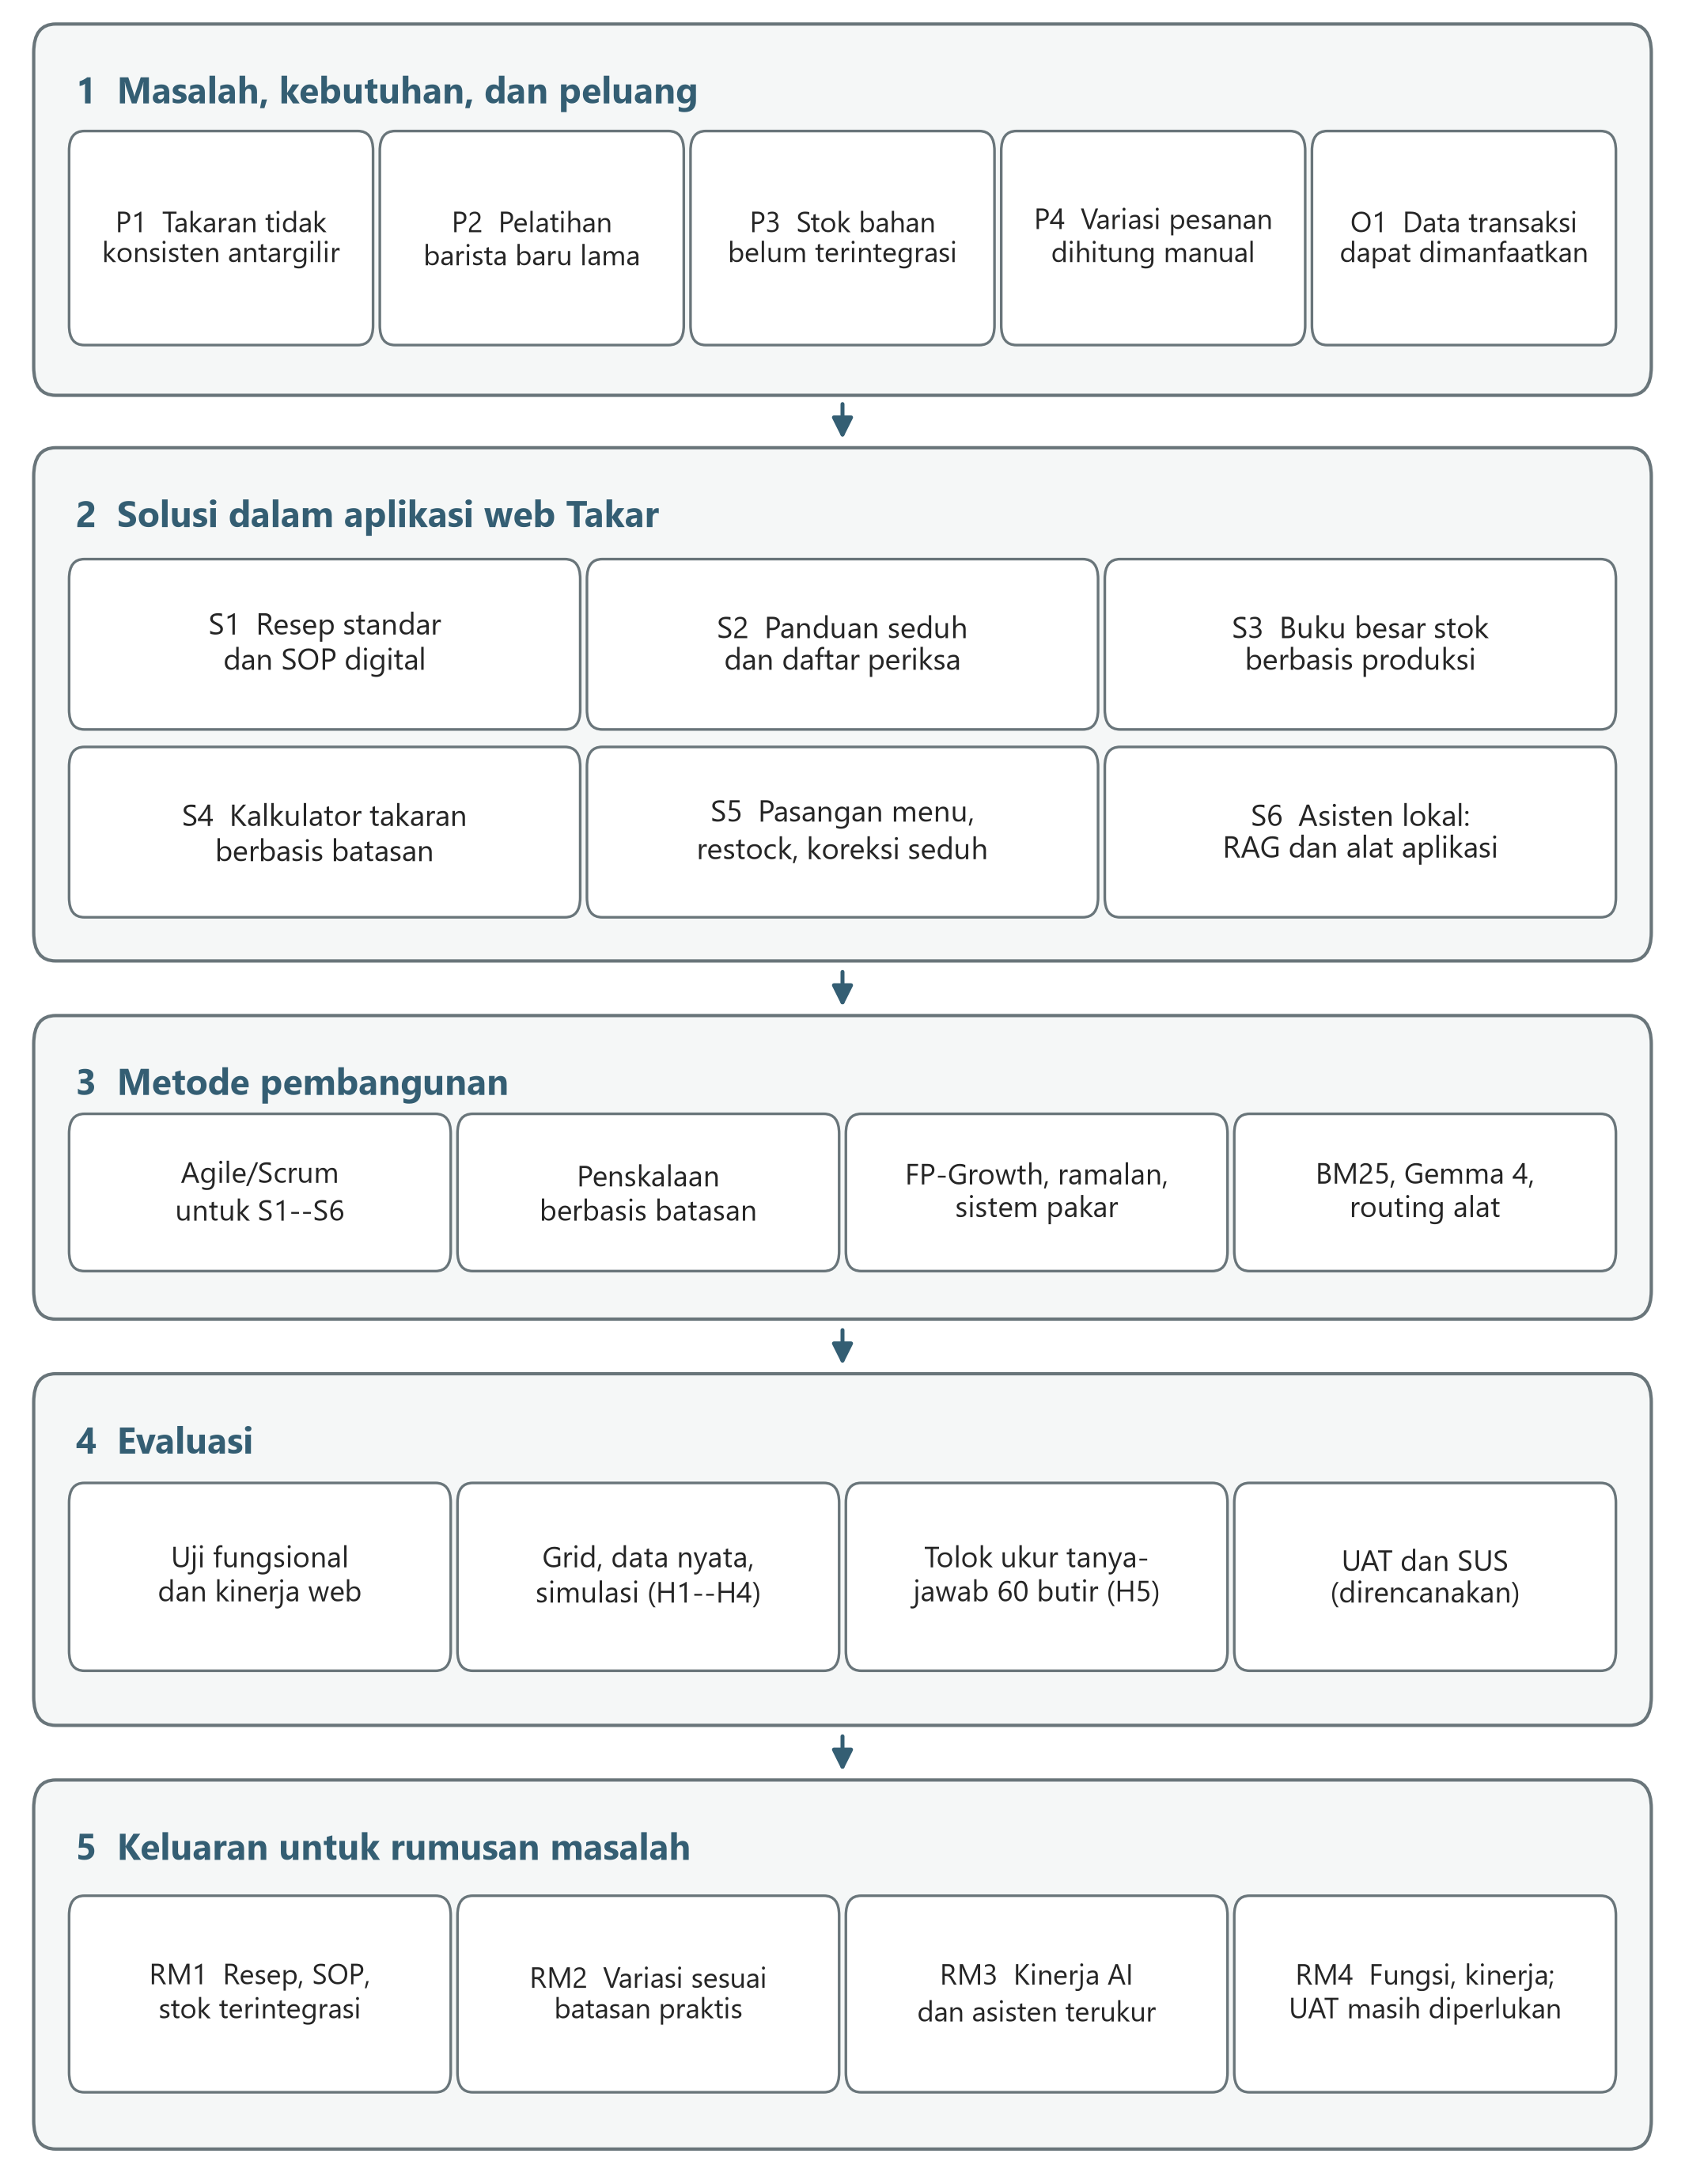
\includegraphics[width=\textwidth]{pic/kerangka_pemikiran.png}
\caption{Kerangka Pemikiran Penelitian}
\label{fig:kerangka-pemikiran}
\end{figure}

Lapis pertama memuat tiga masalah dari arahan, yaitu takaran resep yang tidak konsisten antar-\textit{shift} (P1), pelatihan barista baru yang memakan waktu lama (P2), dan inventaris bahan baku yang belum terintegrasi (P3); satu kebutuhan yang diturunkan penulis dari rumusan masalah arahan tentang kalkulator resep dinamis, yaitu kebutuhan bahan untuk variasi pesanan yang tanpa sistem harus dihitung manual (P4); serta satu peluang, yaitu data transaksi penjualan yang dapat diolah (O1). Lapis kedua memetakan masalah tersebut ke solusi pada aplikasi web Takar. Teori penyeduhan (Subbab~\ref{subsec:penyeduhan}) menunjukkan bahwa mutu seduhan dikendalikan oleh parameter yang dapat diukur, sehingga resep standar dan SOP digital (S1) dapat menjadi acuan yang sama bagi setiap \textit{shift}, sedangkan panduan seduh terpandu dan daftar periksa SOP (S2) berfungsi sebagai alat bantu kerja bagi barista baru (Subbab~\ref{subsec:kedai-kopi}). Buku besar stok yang terhubung ke produksi melalui BOM resep (S3) menjawab P3 (Subbab~\ref{subsec:persediaan}), dan kalkulator takaran dinamis (S4) menjawab P4 dengan penskalaan berbasis batasan karena faktor konversi linier dapat melanggar batasan bar (Subbab~\ref{subsec:penskalaan}). Modul AI operasional (S5) memanfaatkan O1 untuk rekomendasi pasangan menu dan \textit{restock}, serta bagan kendali seduh untuk koreksi parameter seduh. Asisten lokal (S6) membantu barista menemukan pengetahuan dalam resep dan SOP, serta menyerahkan perhitungan kepada layanan aplikasi (Subbab~\ref{subsec:llm-rag}).

Lapis ketiga memuat metode untuk membangun solusi tersebut, yaitu Scrum yang disesuaikan untuk S1--S6 (Subbab~\ref{subsec:scrum}), penskalaan berbasis batasan untuk S4, FP-Growth, peramalan dengan kebijakan persediaan, dan sistem pakar \textit{forward chaining} untuk S5 (Subbab~\ref{subsec:aturan-asosiasi}--\ref{subsec:sistem-pakar}), serta BM25, Gemma 4 lokal, dan pemanggilan alat untuk S6 (Subbab~\ref{subsec:llm-rag}). Lapis keempat memuat pengujian \textit{black-box}, evaluasi algoritma pada data sampel fiktif dan data nyata, tolok ukur tanya-jawab 60 butir untuk H5, pengukuran kinerja, serta UAT dengan SUS yang direncanakan. Lapis kelima memuat hasil untuk setiap rumusan masalah: resep, SOP, dan inventaris terintegrasi (RM1); takaran yang memenuhi batasan praktis (RM2); kinerja modul AI dan asisten yang terukur (RM3); serta pengujian fungsi dan kinerja dengan penerimaan pengguna yang masih perlu diperiksa (RM4).

Rantai argumen tersebut menurunkan lima hipotesis yang telah dirumuskan pada Subbab~\ref{sec:hipotesis}. H1 berasal dari teori penskalaan: algoritma berbasis batasan diharapkan menghindari pelanggaran praktis yang muncul dari penskalaan linier. H2 berasal dari teori aturan asosiasi: FP-Growth semestinya memberi HR@5 lebih tinggi daripada popularitas. H3 berasal dari teori peramalan: model yang dipilih pada data pengembangan semestinya memberi WAPE lebih rendah daripada naif musiman pada data uji. H4 berasal dari teori persediaan: kebijakan berbasis ramalan semestinya menghasilkan \textit{fill rate} lebih tinggi daripada ROP statis. H5 berasal dari teori RAG dan pemanggilan alat: asisten dengan keduanya diharapkan memberi akurasi jawaban lebih tinggi dan angka tanpa dasar lebih sedikit daripada model tanpa konteks pada pertanyaan yang sama. Kelima hipotesis dapat saja tidak didukung data, dan hasilnya dilaporkan apa adanya pada Bab~\ref{bab:hasil}.

% Kembalikan nilai \righthyphenmin untuk bab berikutnya.
\righthyphenmin=\babDuaRightHyphenMin\relax
